\newif\ifshowsolutions
\showsolutionstrue
\input{./preamble}
\DeclareMathOperator*{\argmax}{arg\,max}
\DeclareMathOperator*{\argmin}{arg\,min}


%%%%%%%%%%%%%%%%%%%%%%%%%%%%%%
% HEADER
%%%%%%%%%%%%%%%%%%%%%%%%%%%%%%

\chead{
  {\vbox{
      Machine Learning \& Data Mining \hfill
      Caltech CS/CNS/EE 155 \hfill \\[1pt]
      Miniproject 2\hfill
      February 2025 \\
    }
  }
}

\begin{document}
\pagestyle{fancy}



%%%%%%%%%%%%%%%%%%%%%%%%%%%%%%
% PROBLEM 1
%%%%%%%%%%%%%%%%%%%%%%%%%%%%%%

\newpage

\section{Introduction}
    \begin{itemize}
        \item Team Name: jc
        \item Group members: Chenning Xu, Joahan Casta\~{n}eda Jaimes
        \item Division of labor:
        \item Packages used: suprise, numpy, matplotlib
    \end{itemize} 
\newpage

\section{Basic Visualizations}
Our group produced the following histograms for the MovieLens dataset:
\begin{figure}[H]
    \centering 
    \includegraphics[width=\textwidth]{2x3hist.png}
\end{figure}
We noticed that the most common rating that was given to a film was a rating of 4. The distribution as a whole is left skewed with a 
mean value of 3.53. One might have suspected that a rating scale of 1 to 5 would yield a mean rating of 3, but it appears that this rating 
distribution does not obey a normal distribution.
\par 
The shape of the ratings distribution for the most popular movies is similar to the rating distribution of the whole dataset. The mean is slightly 
higher and there are now more 5 ratings than 3 ratings. Therefore the popular movies tend to have higher ratings as a whole, but not by an absurdly 
noticable amount. This is what our group expected to see.
\par 
There are only ratings of 5 on this histogram for the 10 highest rated movies since the movies with the highest ratings are those which have had 
very few users rate them and rate them very highly (as is indicated by the lower frequency counts). This is what we would expect.
\par 
For our three genres, we selected ``Crime,'' ``Horror,'' and ``Western.'' Crime movies were the most popular and were marginally the highest rated 
genre of the three that we chose. Horror moves were the second most popular and were by far the lowest rated genre of the three. Finally, Western 
moves were the least popular but were comparable in mean rating to the movies in the Crime genre.
\newpage

\section{Matrix Factorization Visualizations}

\subsection{Model training and explanation}

In the first model that we trained, we following the factorization procedure that was outlined in Set 5. To derive the coefficients of the matricies 
$U \in \mathbb{R}^{M\times K}$ and $V \in \mathbb{R}^{N\times K}$, we minimize the regularized square error as defined by the following objective:
\begin{equation}
    \argmin \frac{\lambda}{2}\left(||U||^2_F + ||V||^2_F\right) + \frac{1}{2}\sum_{i, j}(y_{ij} - u_i^Tv_j)^2,
\end{equation}
where $u_i^T$ and $v_j^T$ are the row components of $U$ and $V$ and the terms inside the first parentheses correspond to the Frobenium norms of 
the two matricies. This gives rise to a final matrix $Y = UV^T$ where $y_{ij} \approx u_i^Tv_j$. To minimize this objective, stochastic gradient 
descent is utilizied with the following rule updates:
\begin{align}
    u_i = u_{i} - \eta\partial_{u_{i}}, \\
    v_j = v_{j} - \eta\partial_{v_{j}}.
\end{align}
Stochastic gradient descent is stopped once the relative loss reduction compared to the first epoch is beneath some threshold $\epsilon$:
\begin{equation}
    \Delta_{t - 1, t}/\Delta_{0, 1} \le \epsilon.
\end{equation}
\par 
In the second model that we trained, we introduced bias terms $a$ and $b$ to the procedure outlined in Set 5. With these new terms, we now 
minimize the following objective:
\begin{equation}
    \argmin{_{U, V}}\frac{\lambda}{2}\left(||U||^2_F + ||V||^2_F\right) + \frac{1}{2}\sum_{i, j}(y_{ij} - (u_i^Tv_j + a_i + b_j))^2.
\end{equation}
We otherwise use the same gradient descent procedure as is used in the first model, only now we must include the update rules for $a$ and 
$b$:
\begin{align}
    a_i = a_{i} - \eta\partial_{a_{i}}, \\
    b_j = b_{j} - \eta\partial_{b_{j}}.
\end{align}
\par 
For the off-the-shelf implementation, we used the \texttt{surprise} package.

\subsection{Model parameters and performance}

Our model performances are listed in the following table:
\begin{center}
    \begin{tabular}{|c|c|c|}
        \hline
        Model & $E_{in}$ & $E_{out}$ \\ 
        \hline
        SVD w/o bias & 0.336 & 0.454 \\
        \hline
        SVD w/ bias & 0.276 & 0.446 \\ 
        \hline
        SVD (\texttt{surprise}) & 0.873 & 0.920 \\
        \hline
    \end{tabular}
\end{center}

For the standard SVD model with no bias terms, we tuned our model to an early stopping criterion of $\epsilon = 0.001$, a learning rate of $0.03$, 
and a regularization value of $0.1$. These values were used as they minimized overfitting, as was evident in Problem 2 of Homework Set 5. We found 
that very similar parameters were effective to the SVD with the nearly introduced bias terms. We used the same parameters, with the exception of 
the regularization parameter which we found to be most effective at $0.09$.
\par 
Finally for the \texttt{surprise} implementation of SVD, we performed a GridSearch of the model parameter space to tune our model on the
dataset. We used default values for the \texttt{surprise} implementation of SVD except for the learning rate and regularization parameter, which 
we found to be best selected as $0.0264$ and $0.113$, respectively. This implementation has the worst error for both the training set and testing 
set.

\section{Model visualizations}

\subsection{Random ten movies}

\begin{figure}[H]
    \centering
    \subfloat{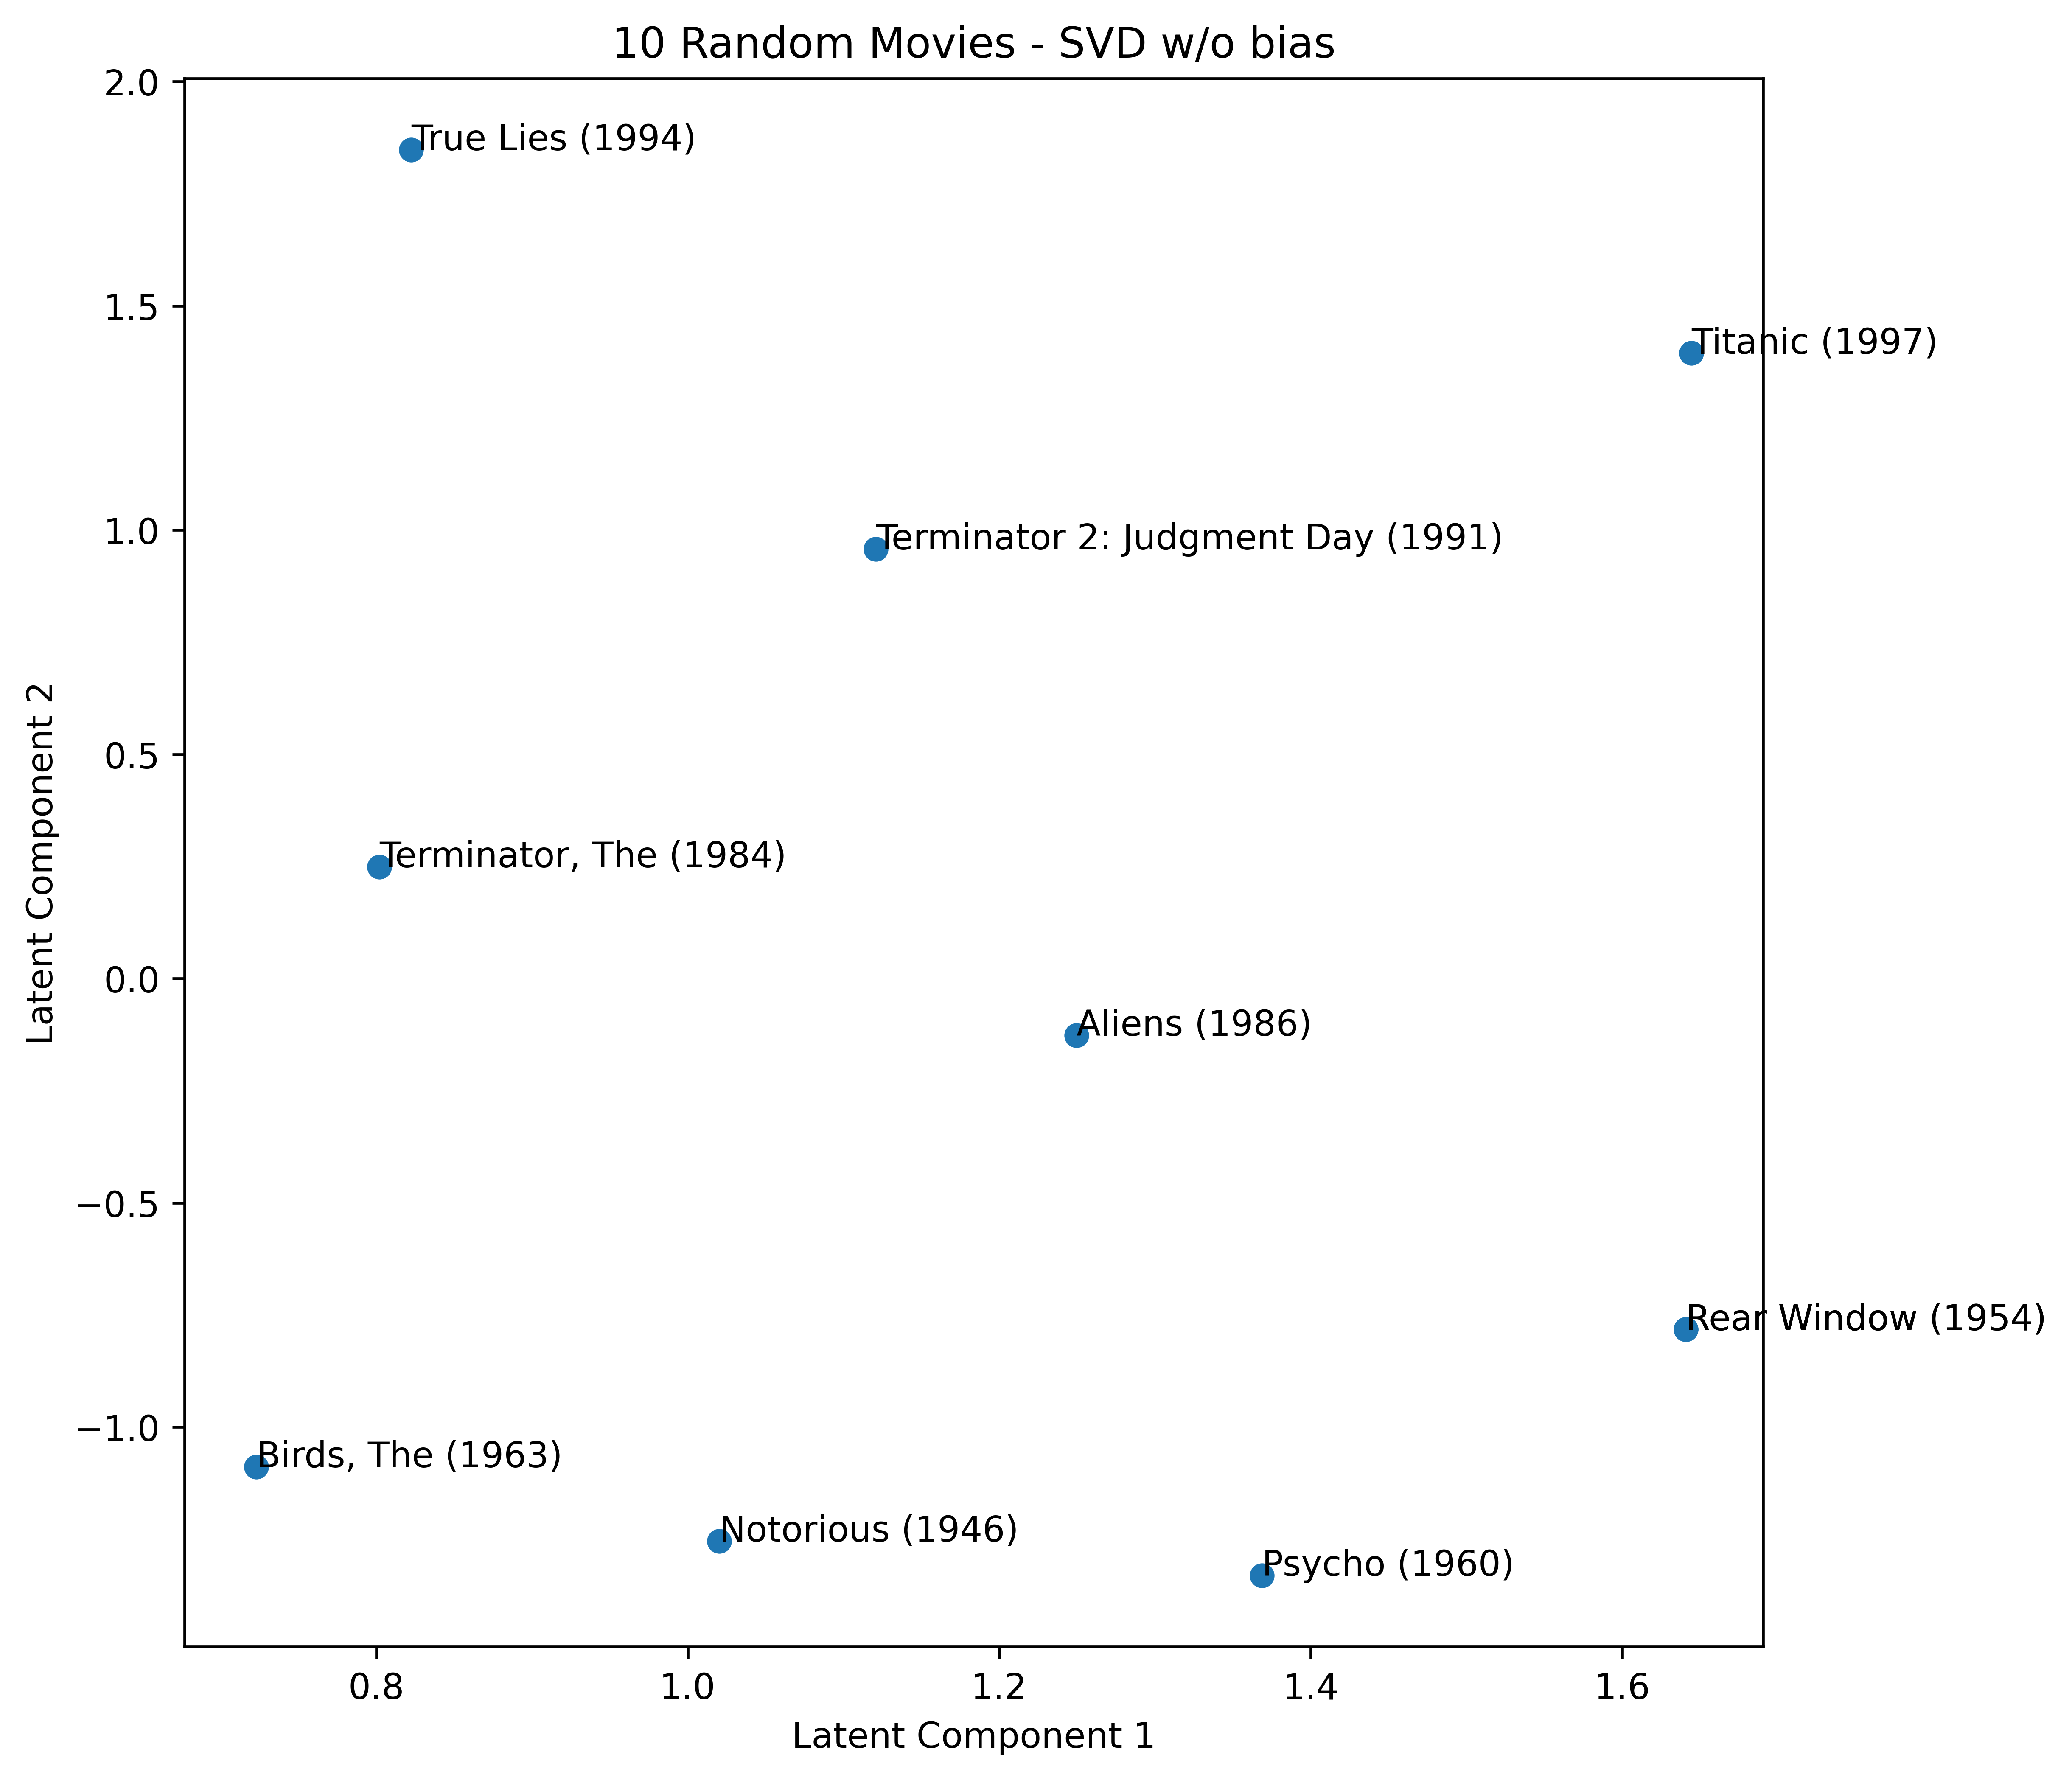
\includegraphics[width = 0.45\textwidth]{rand10_SVD.png}}
    \subfloat{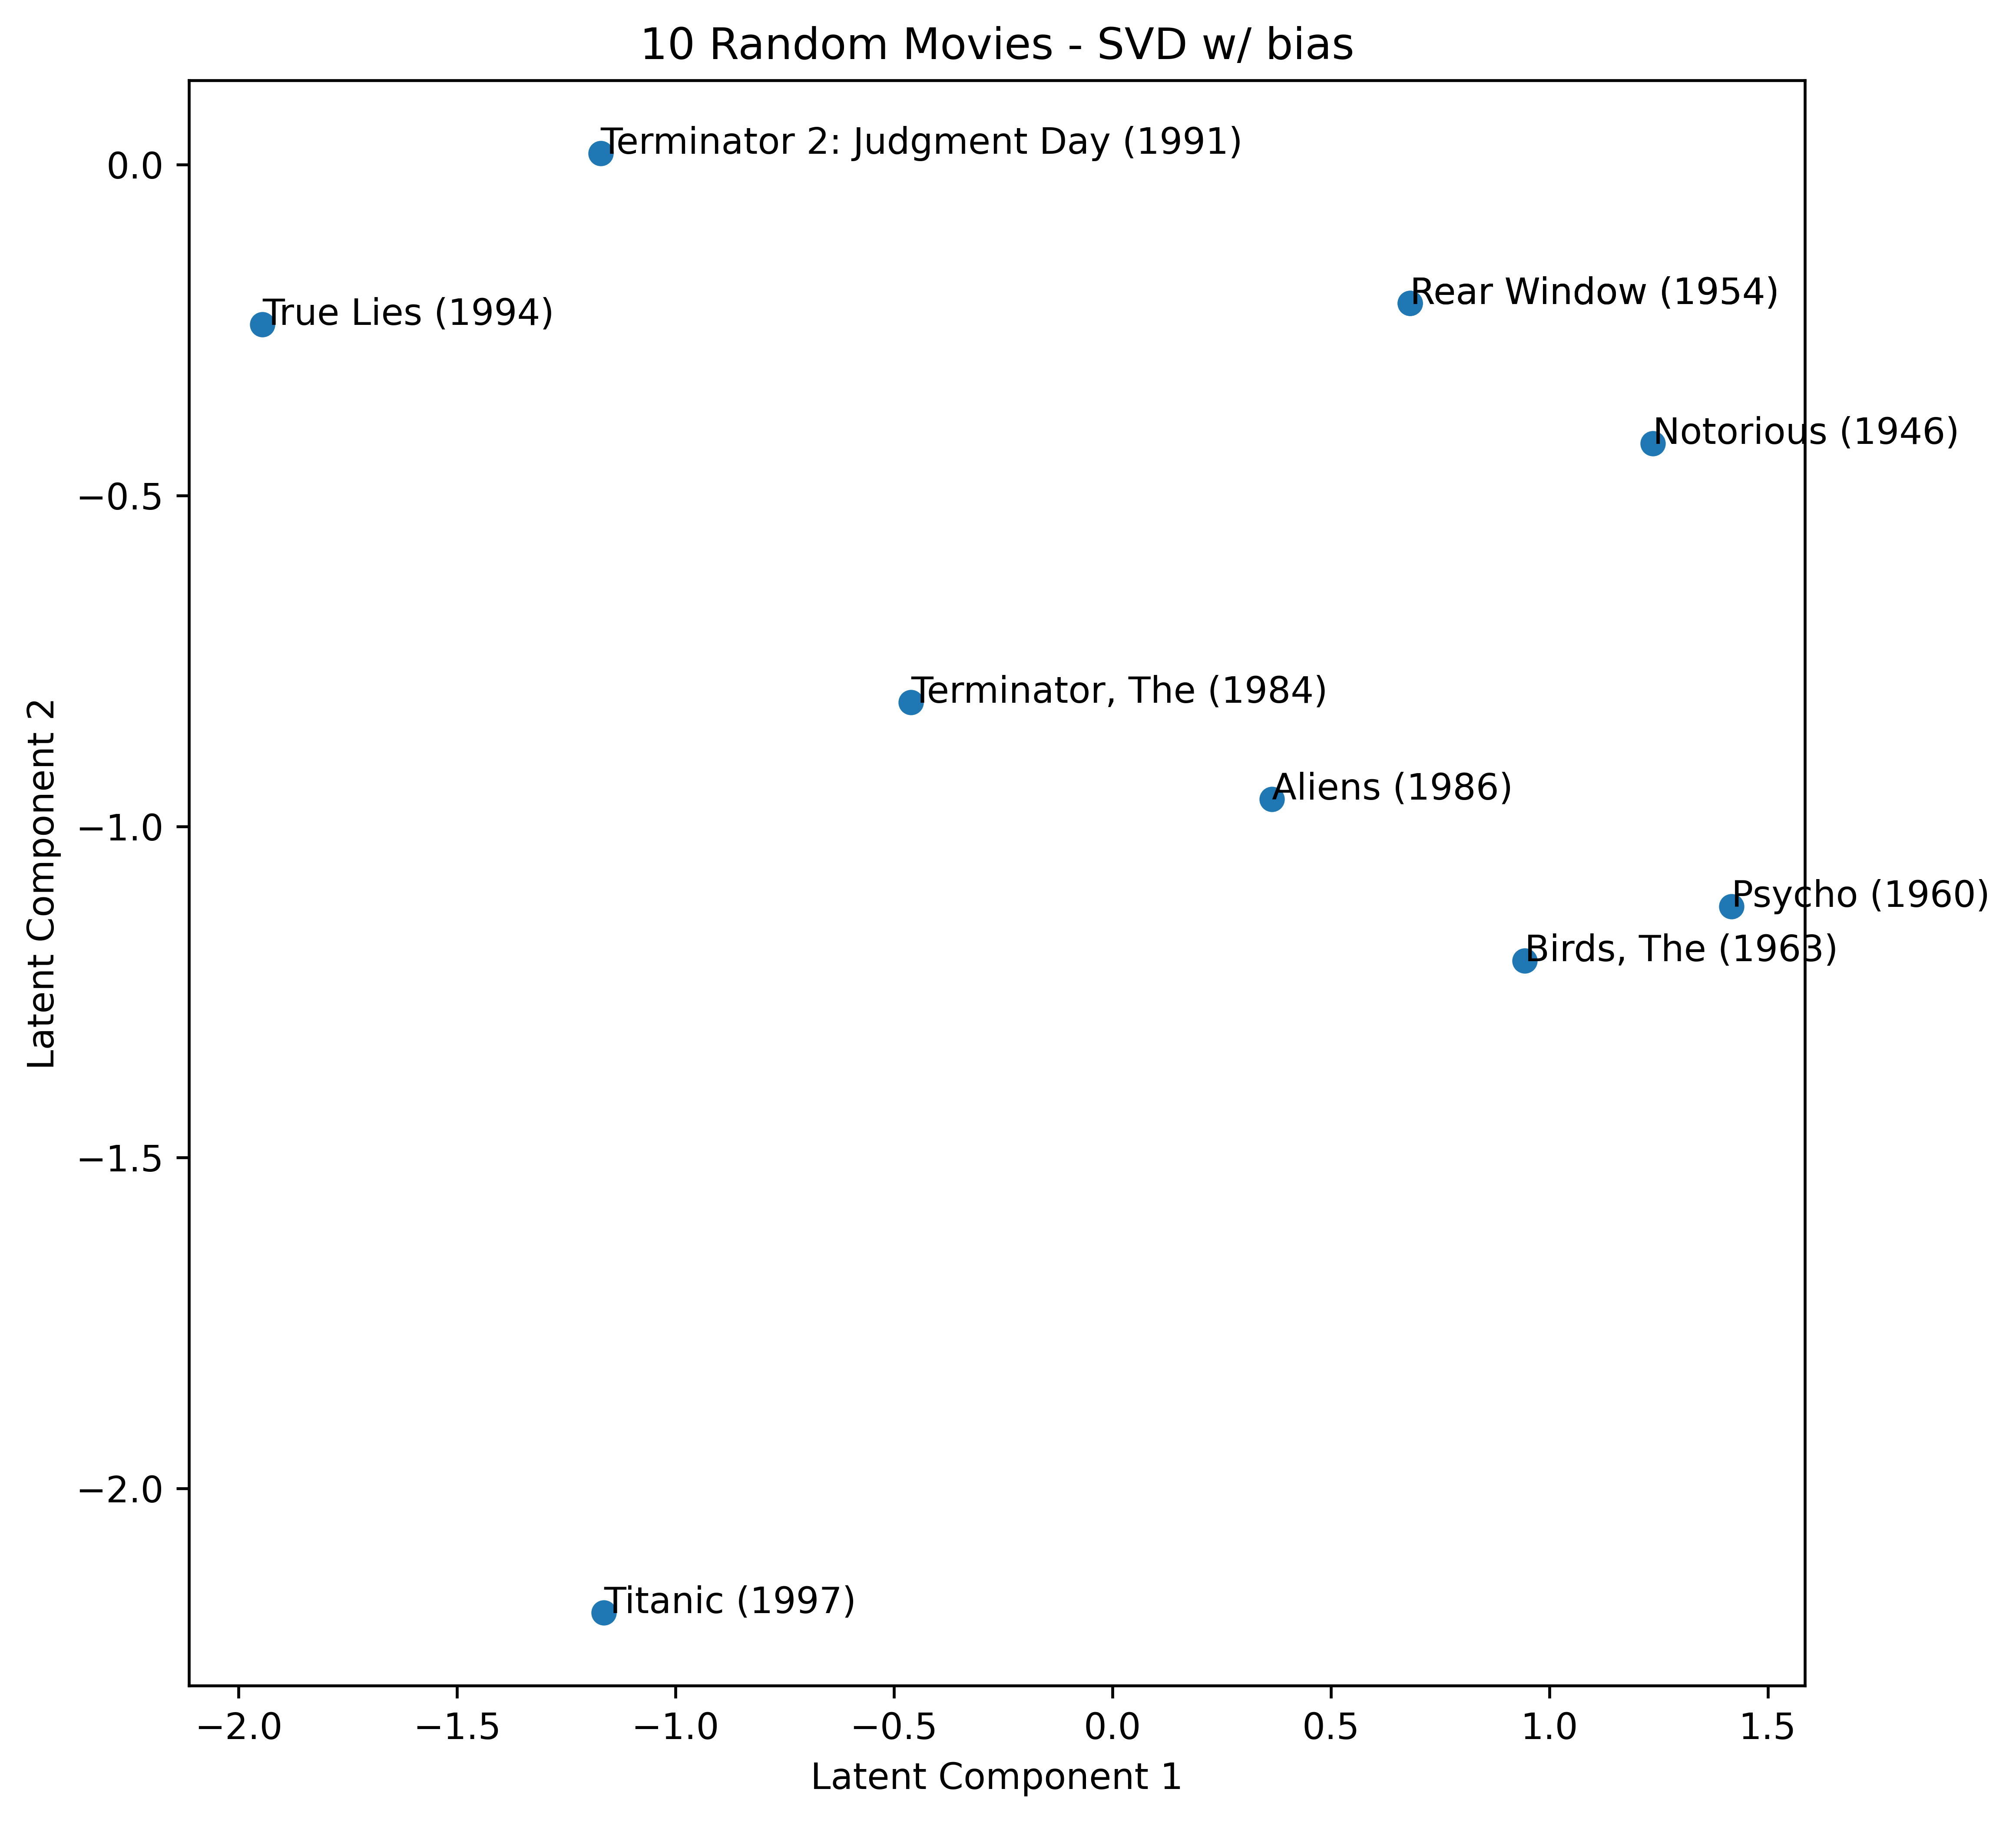
\includegraphics[width = 0.45\textwidth]{rand10_biased.png}}
\end{figure}
\begin{figure}[H]
    \centering 
    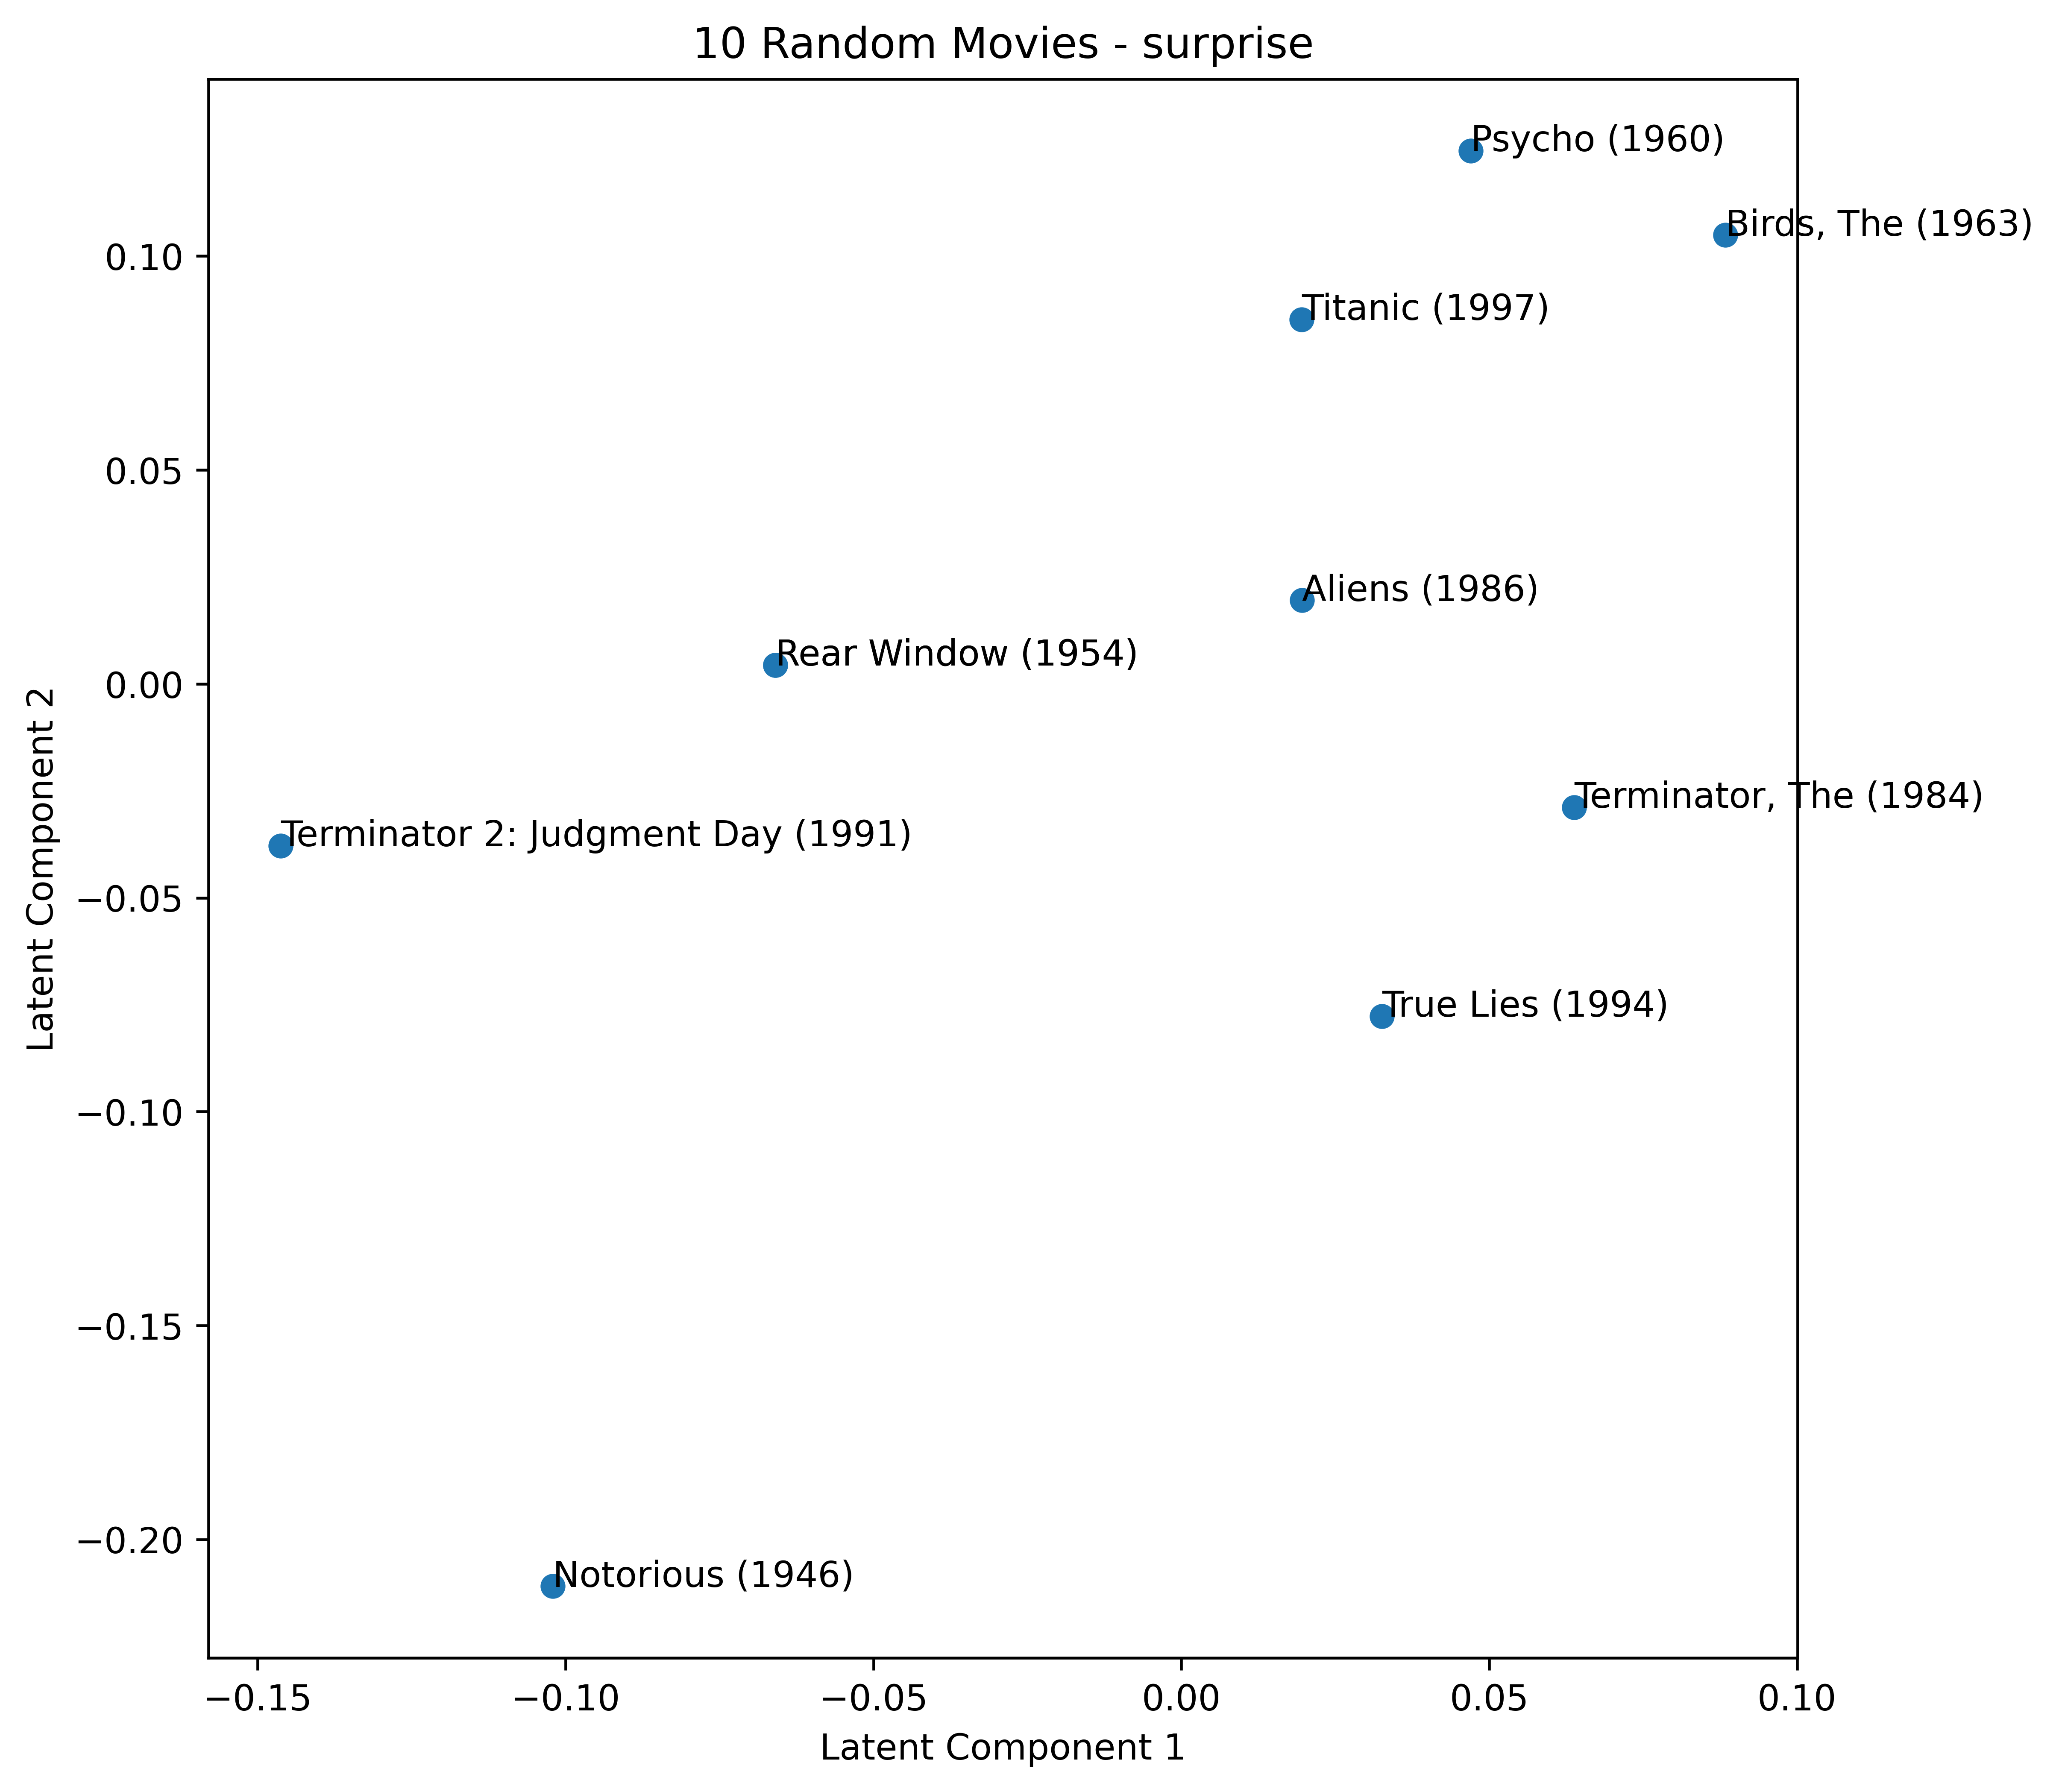
\includegraphics[width=10cm]{rand10_sp.png}
\end{figure}

These are the films that we used for our Piazza post. 10 films were selected, 6 of which were Alfred Hitchcock filsm and 
4 of which are James Cameron films. \textit{Aliens}, \textit{True Lies}, \textit{The Terminator}, and \textit{The Terminator 2} are roughly clustered together in 
the SVD plots of our own implementation with the association being marginally stronger in the model with the bias terms. Our SVD with bias 
identified \textit{Titanic} as an outlier, something that may have to do with its extreme popularity. This model also captures the similar 
themes between \textit{The Birds} and \textit{Psycho}, both being Mystery/Horror films, something that the \texttt{surprise} model also appears 
to capture.
\par 
In the \texttt{surprise} model, \texttt{Notorious} is captured as an outlier, perhaps owing to its abnormally old age among the rest of the films. 
Otherwise, we don't note a significant difference between it and the other SVD implementations. Perhaps we could argue that the SVD plot without 
the bias terms has spread out the points more than the other models, but that's about it. 

\subsection{Ten most highly rated movies}

\begin{figure}[H]
    \centering
    \subfloat{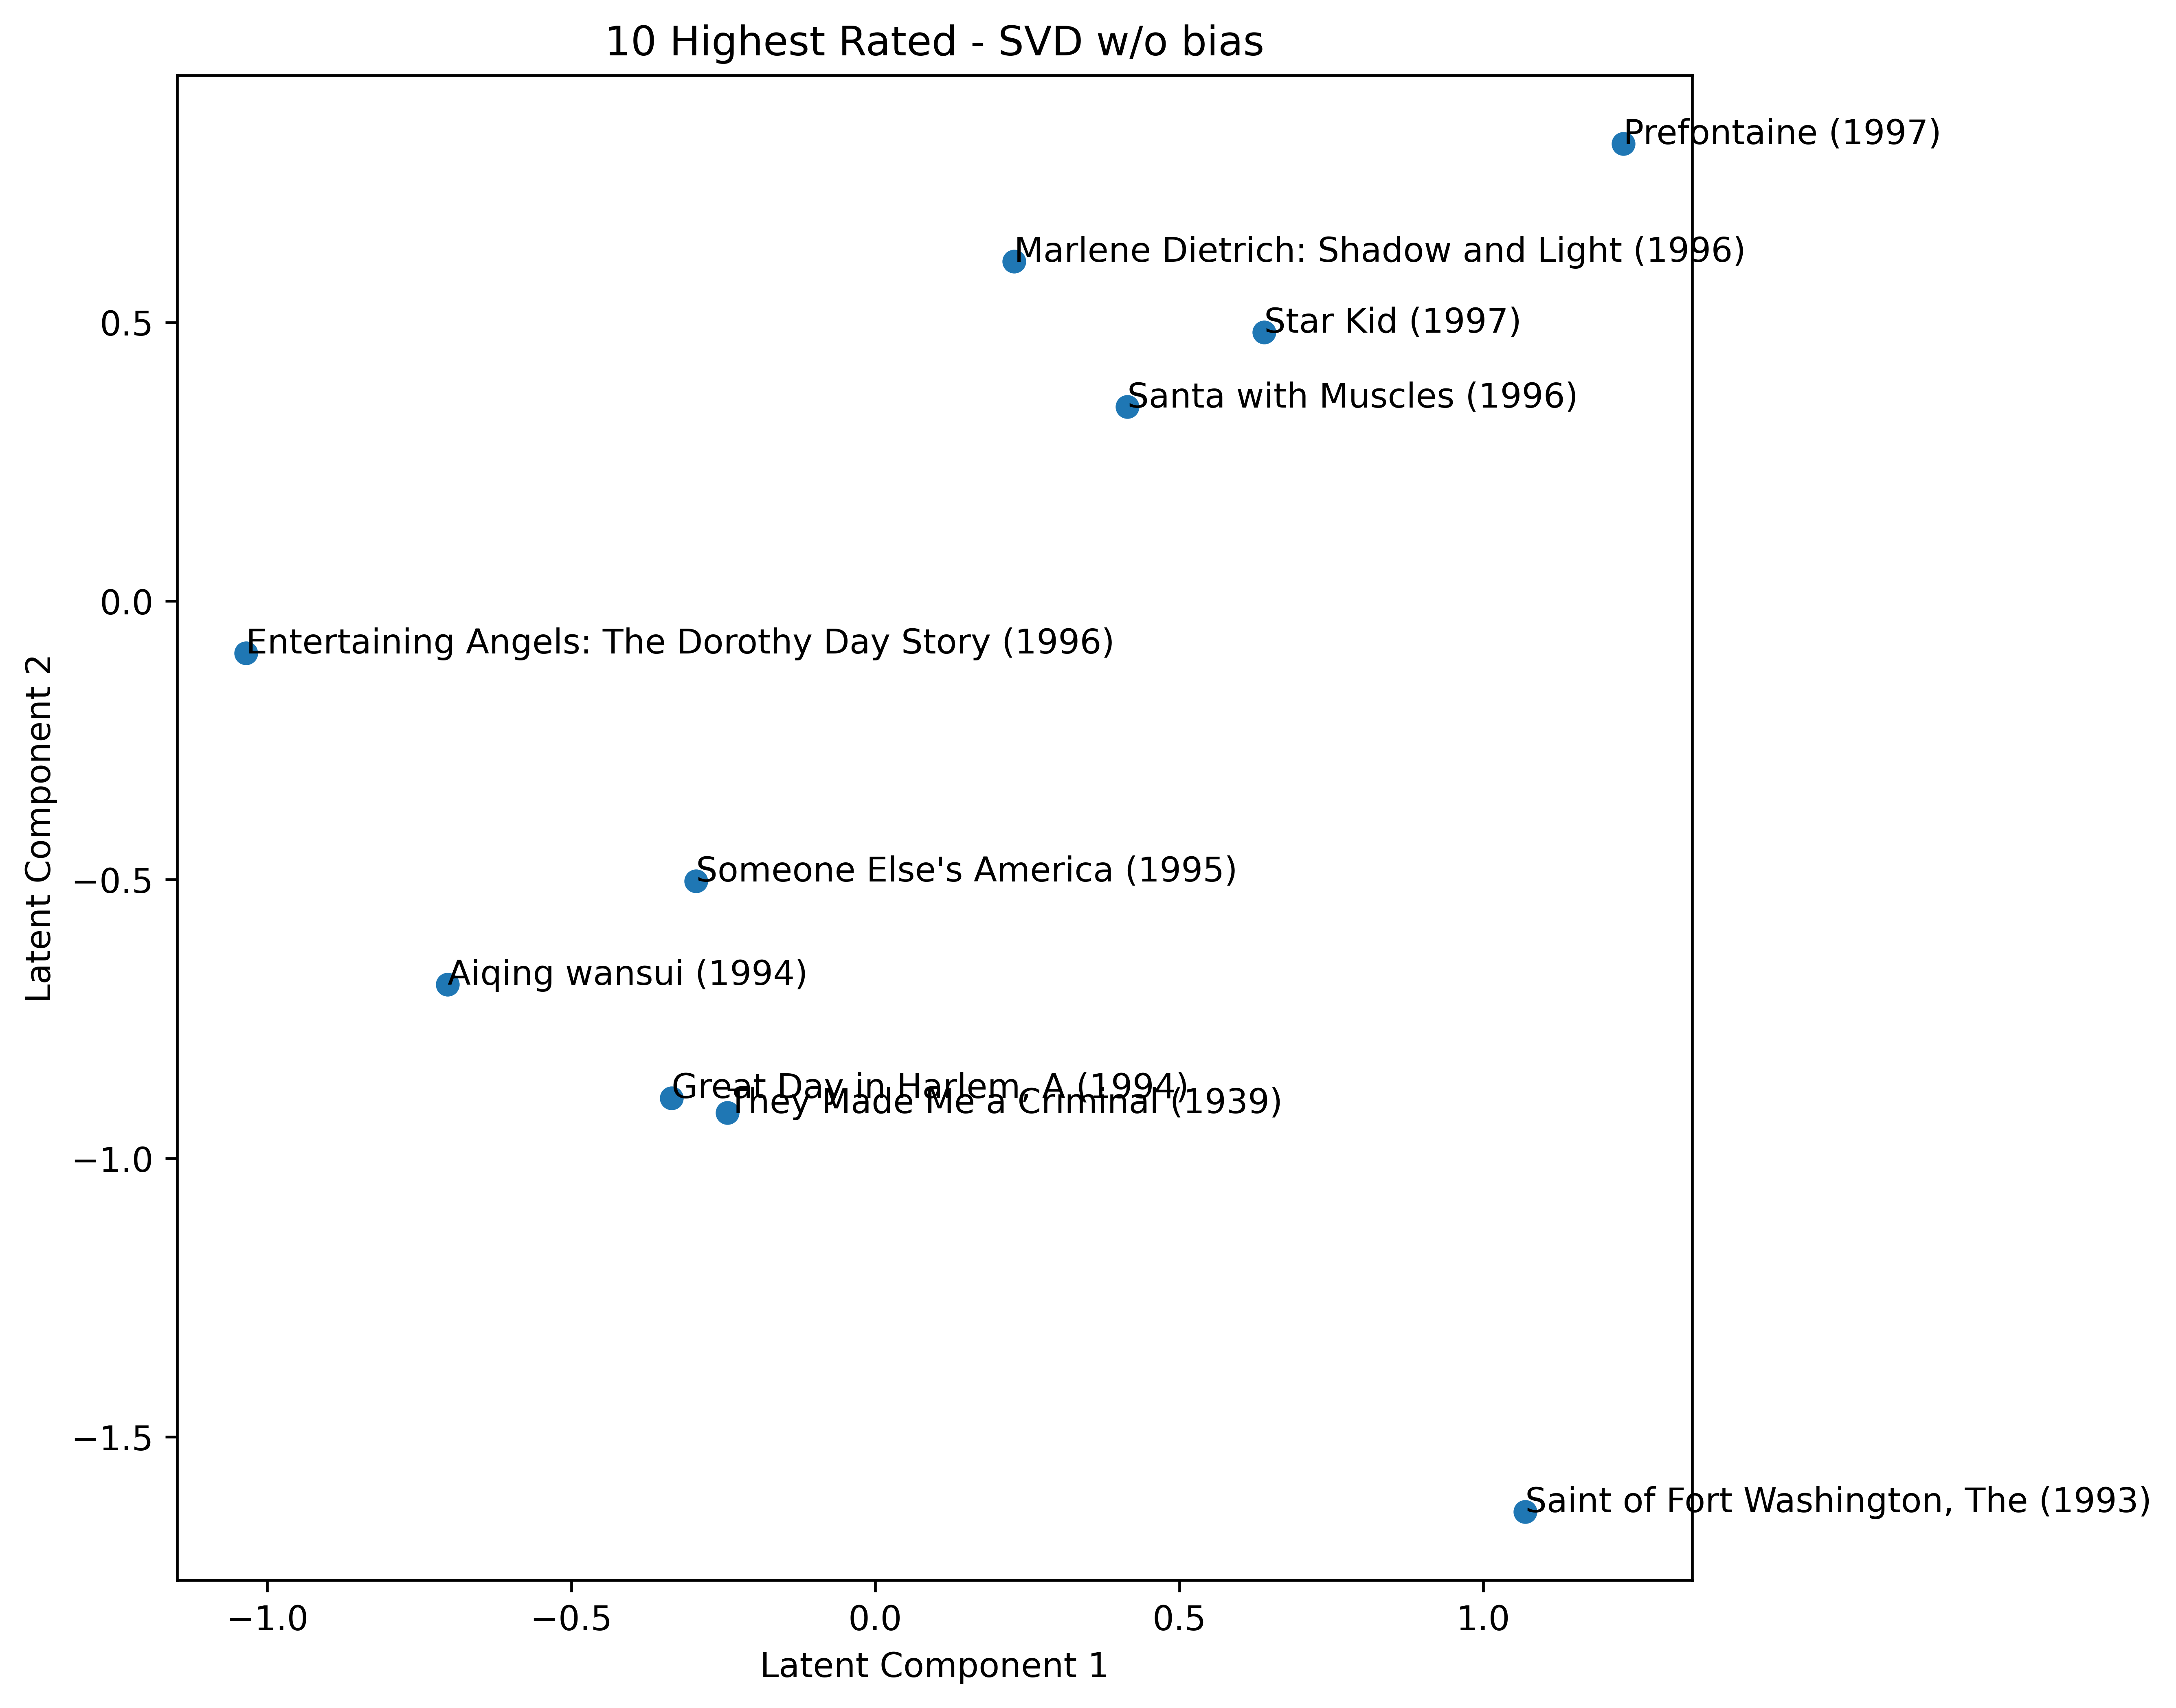
\includegraphics[width = 0.45\textwidth]{most10_SVD.png}}
    \subfloat{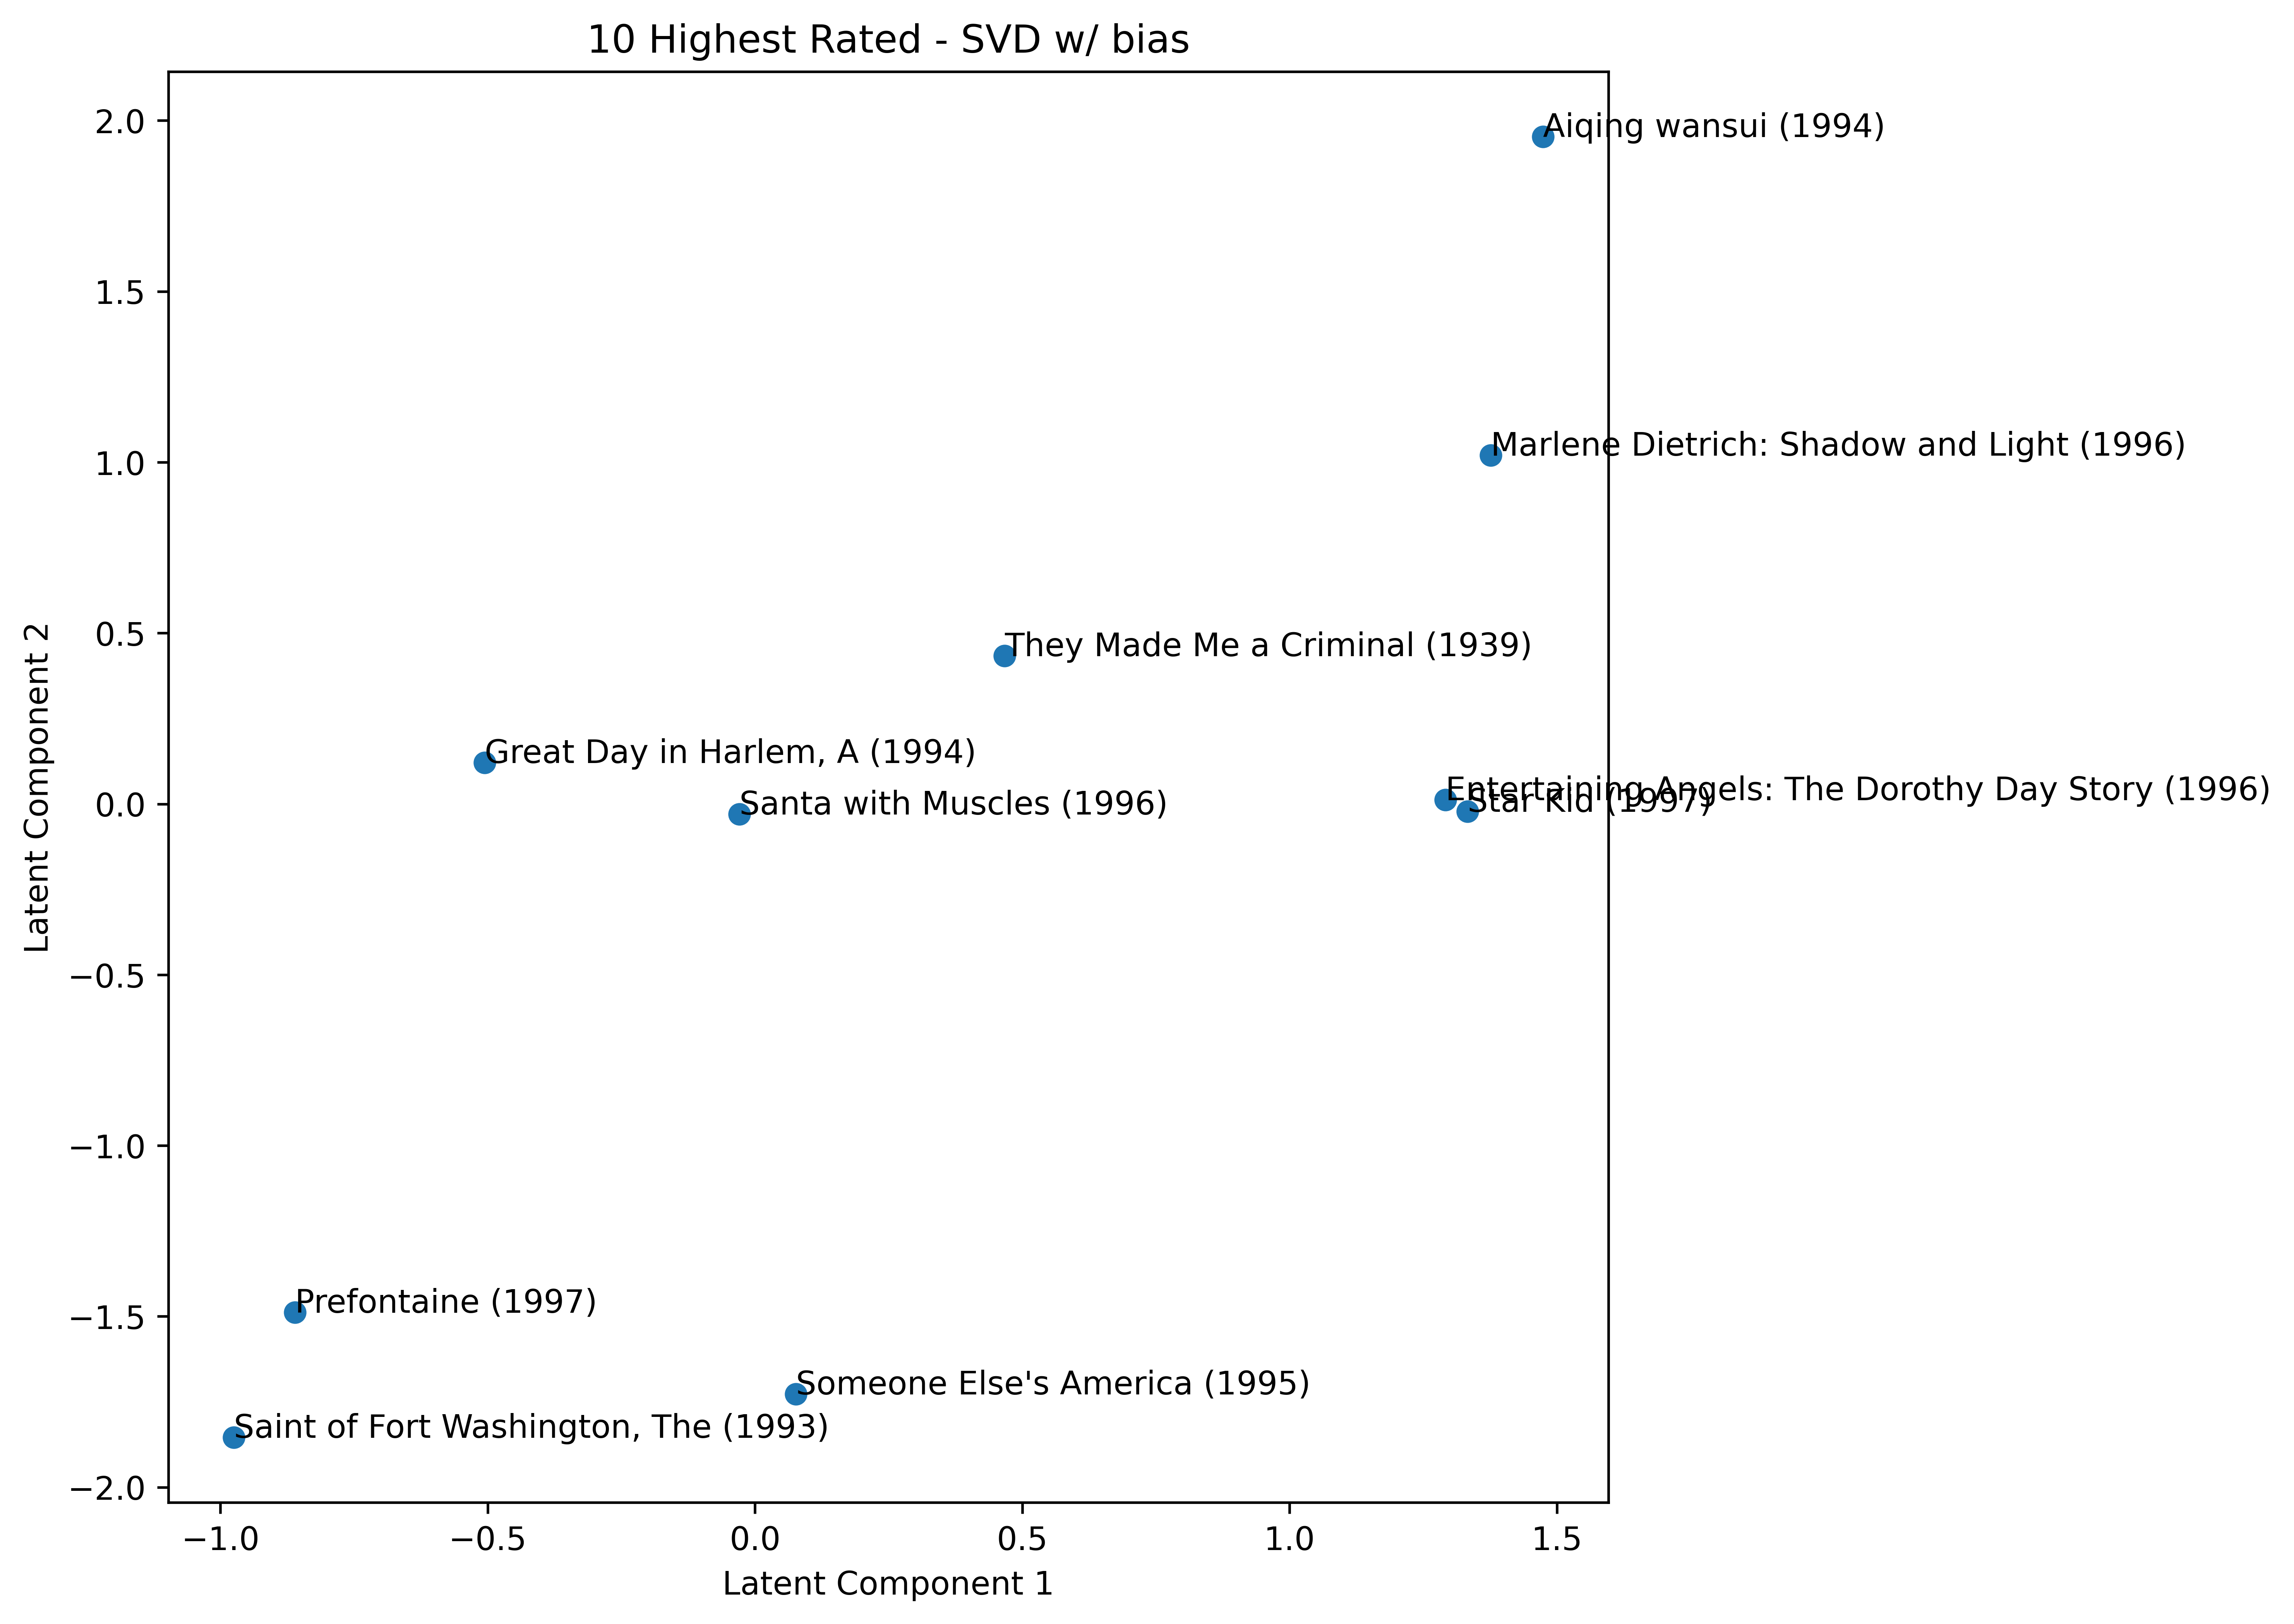
\includegraphics[width = 0.45\textwidth]{most10_biased.png}}
\end{figure}
\begin{figure}[H]
    \centering 
    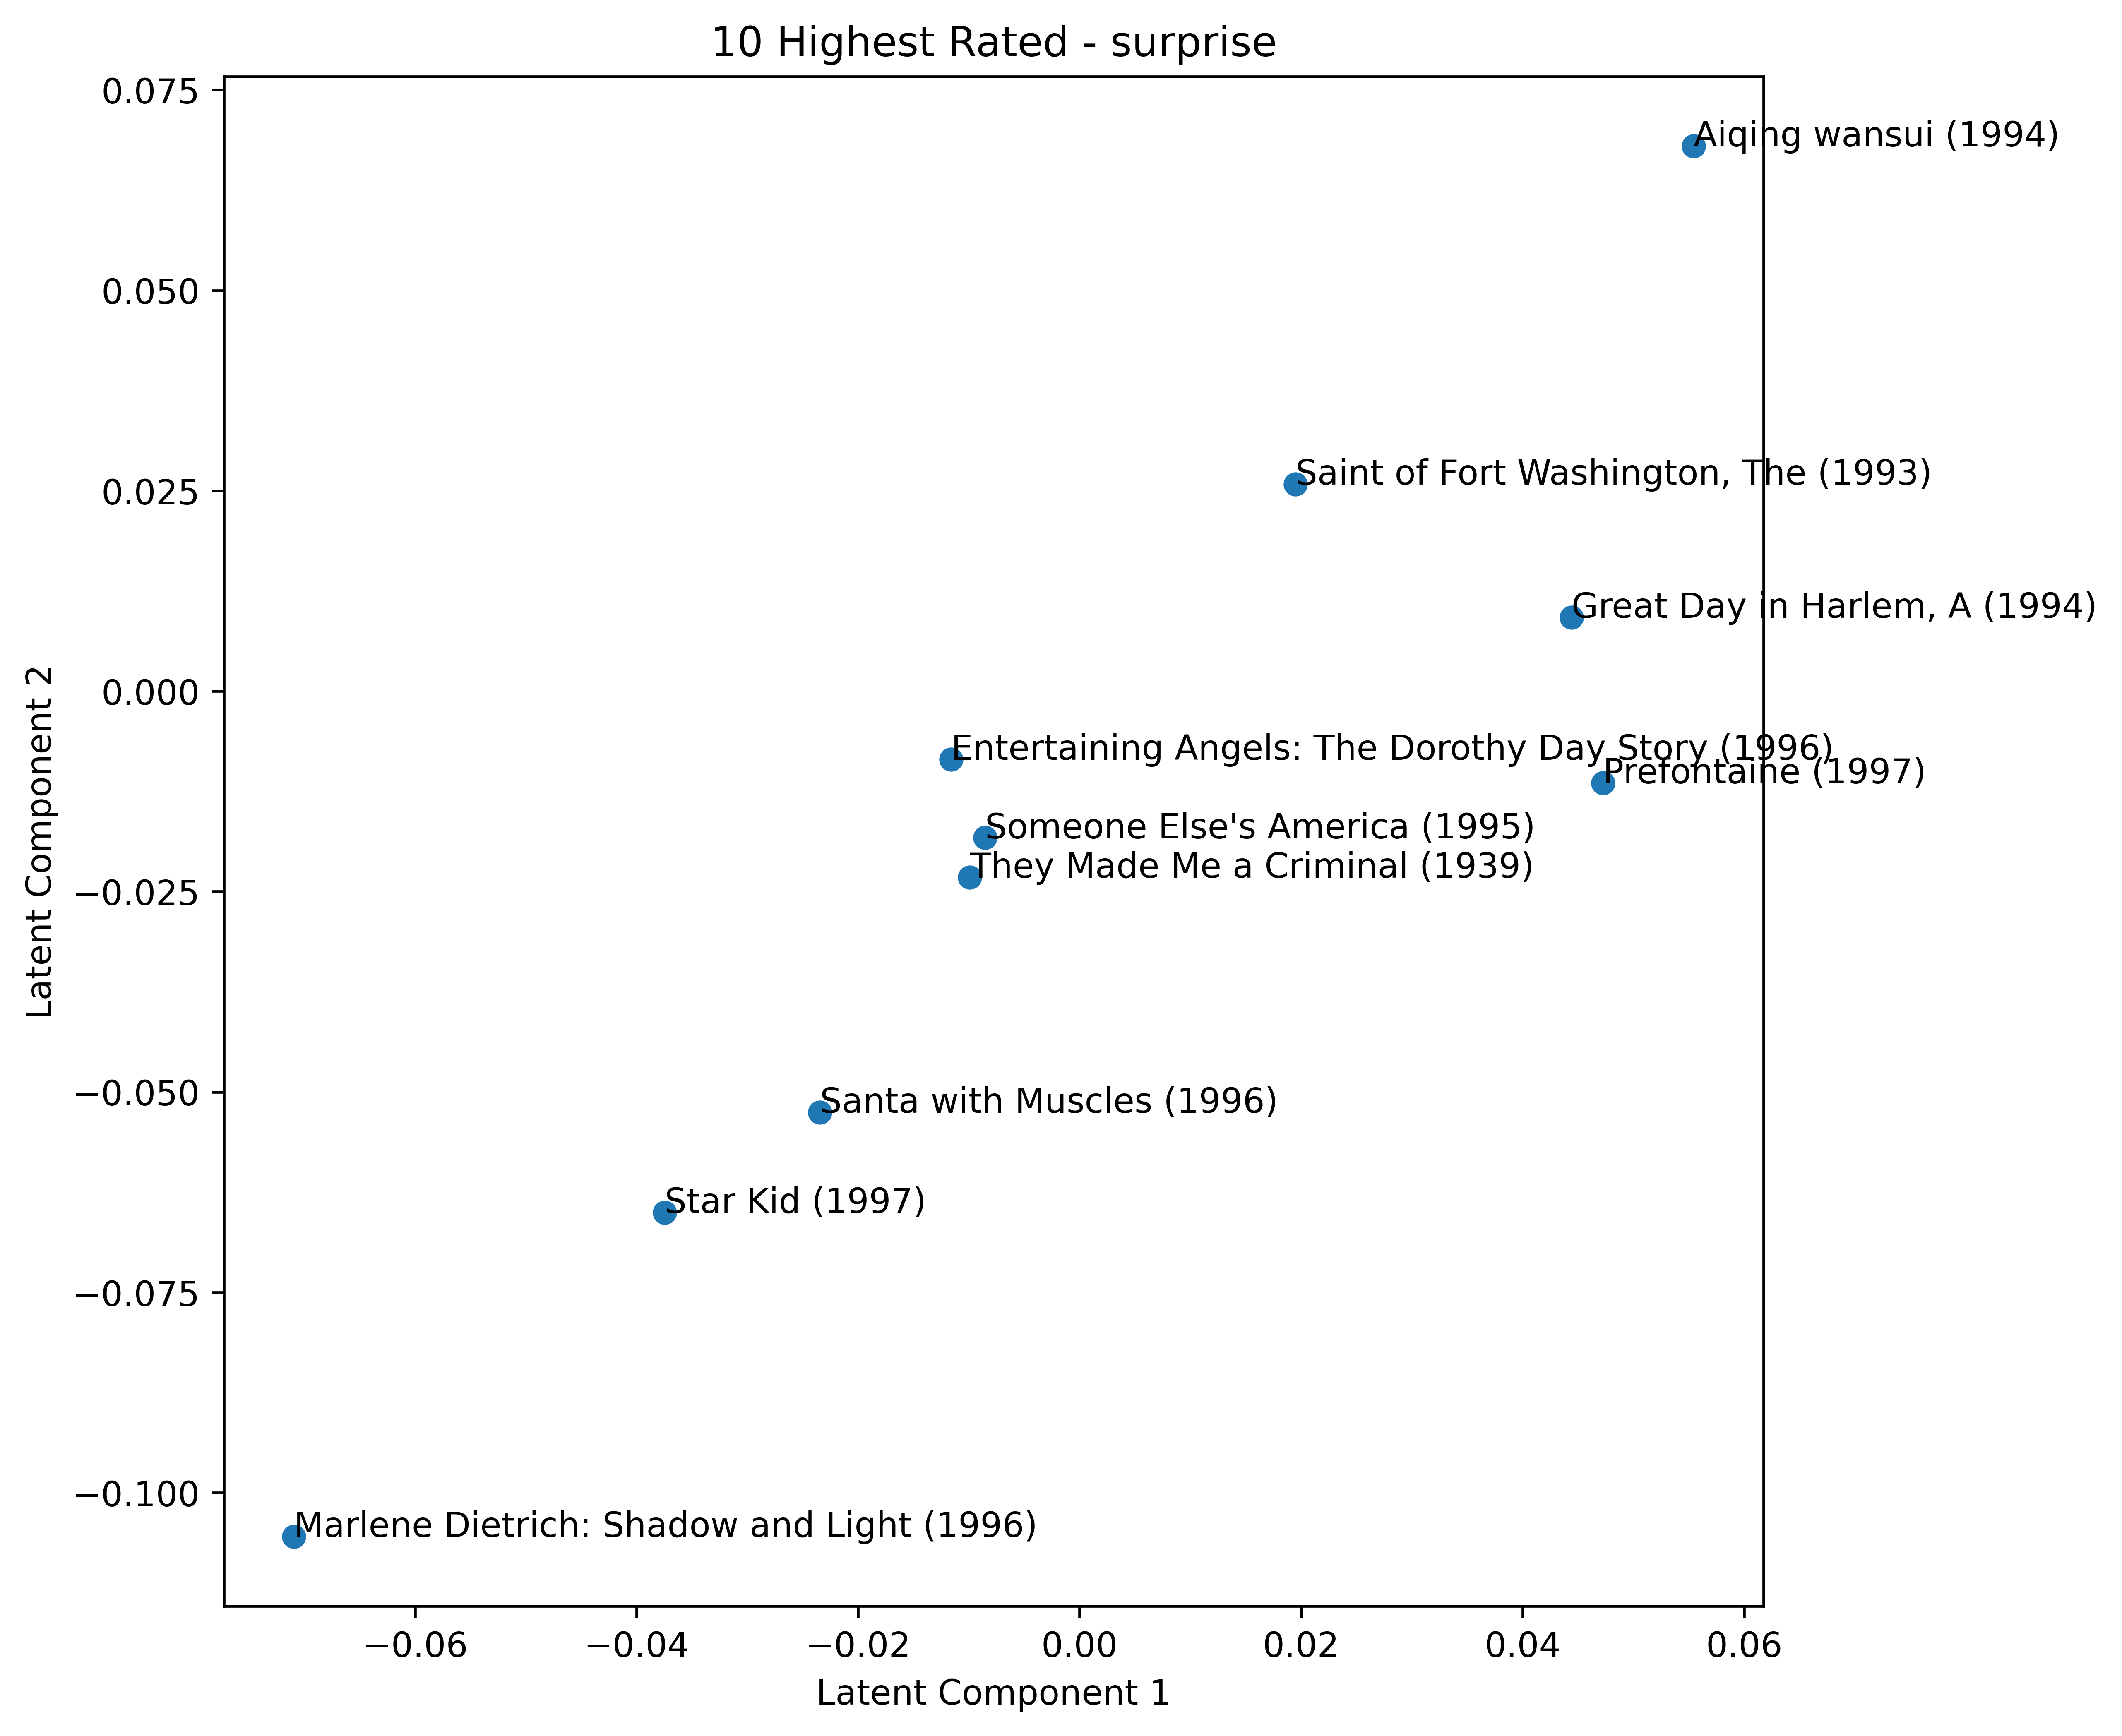
\includegraphics[width=10cm]{most10_sp.png}
\end{figure}

These films do not have a significant amount of ratings and may struggle with correlating well with other similar films in these plots. Despite this, 
\textit{aiqing wansui} stands out as an outlier in the biased SVD implementation and the \texttt{surprise} implementation. This film is Taiwanese, 
the only foreign film in this set of films so that could be why its placed in this particular way. We don't really note any significant correlations 
between films in any implementation, understandably so since these films don't really have as many data points to train on.

\subsection{Ten most popular movies}

\begin{figure}[H]
    \centering
    \subfloat{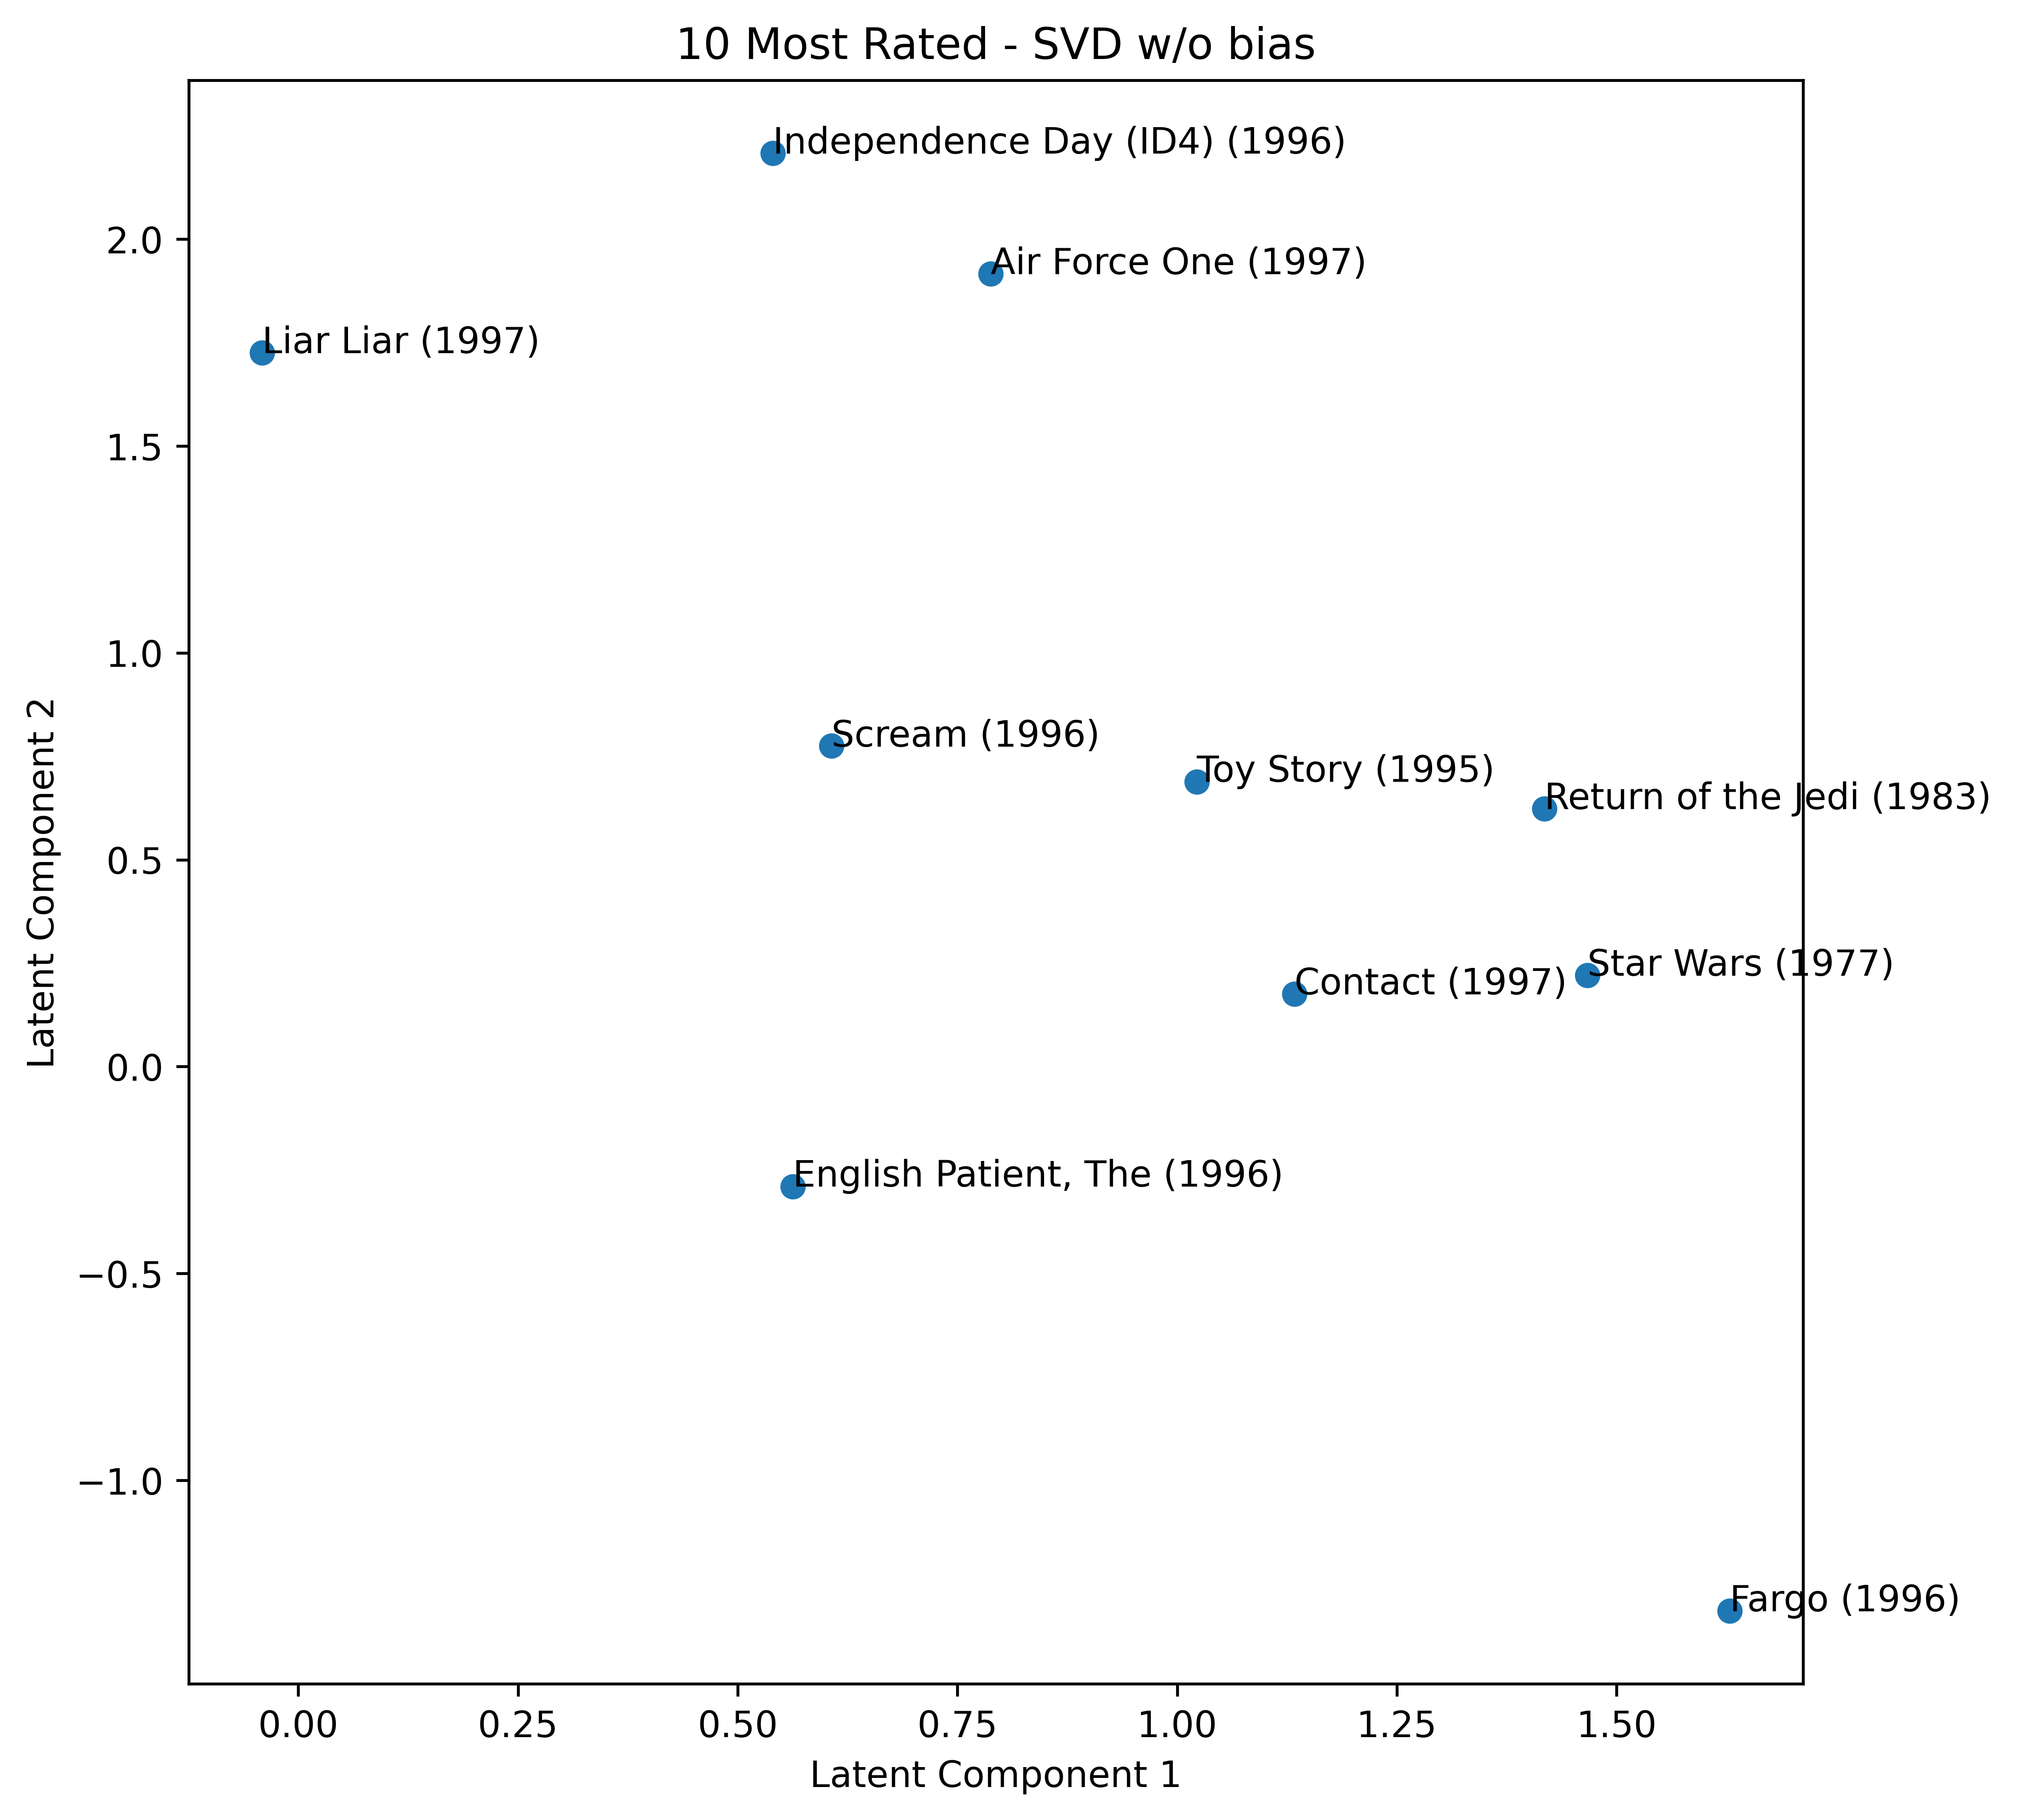
\includegraphics[width = 0.45\textwidth]{pop10_SVD.png}}
    \subfloat{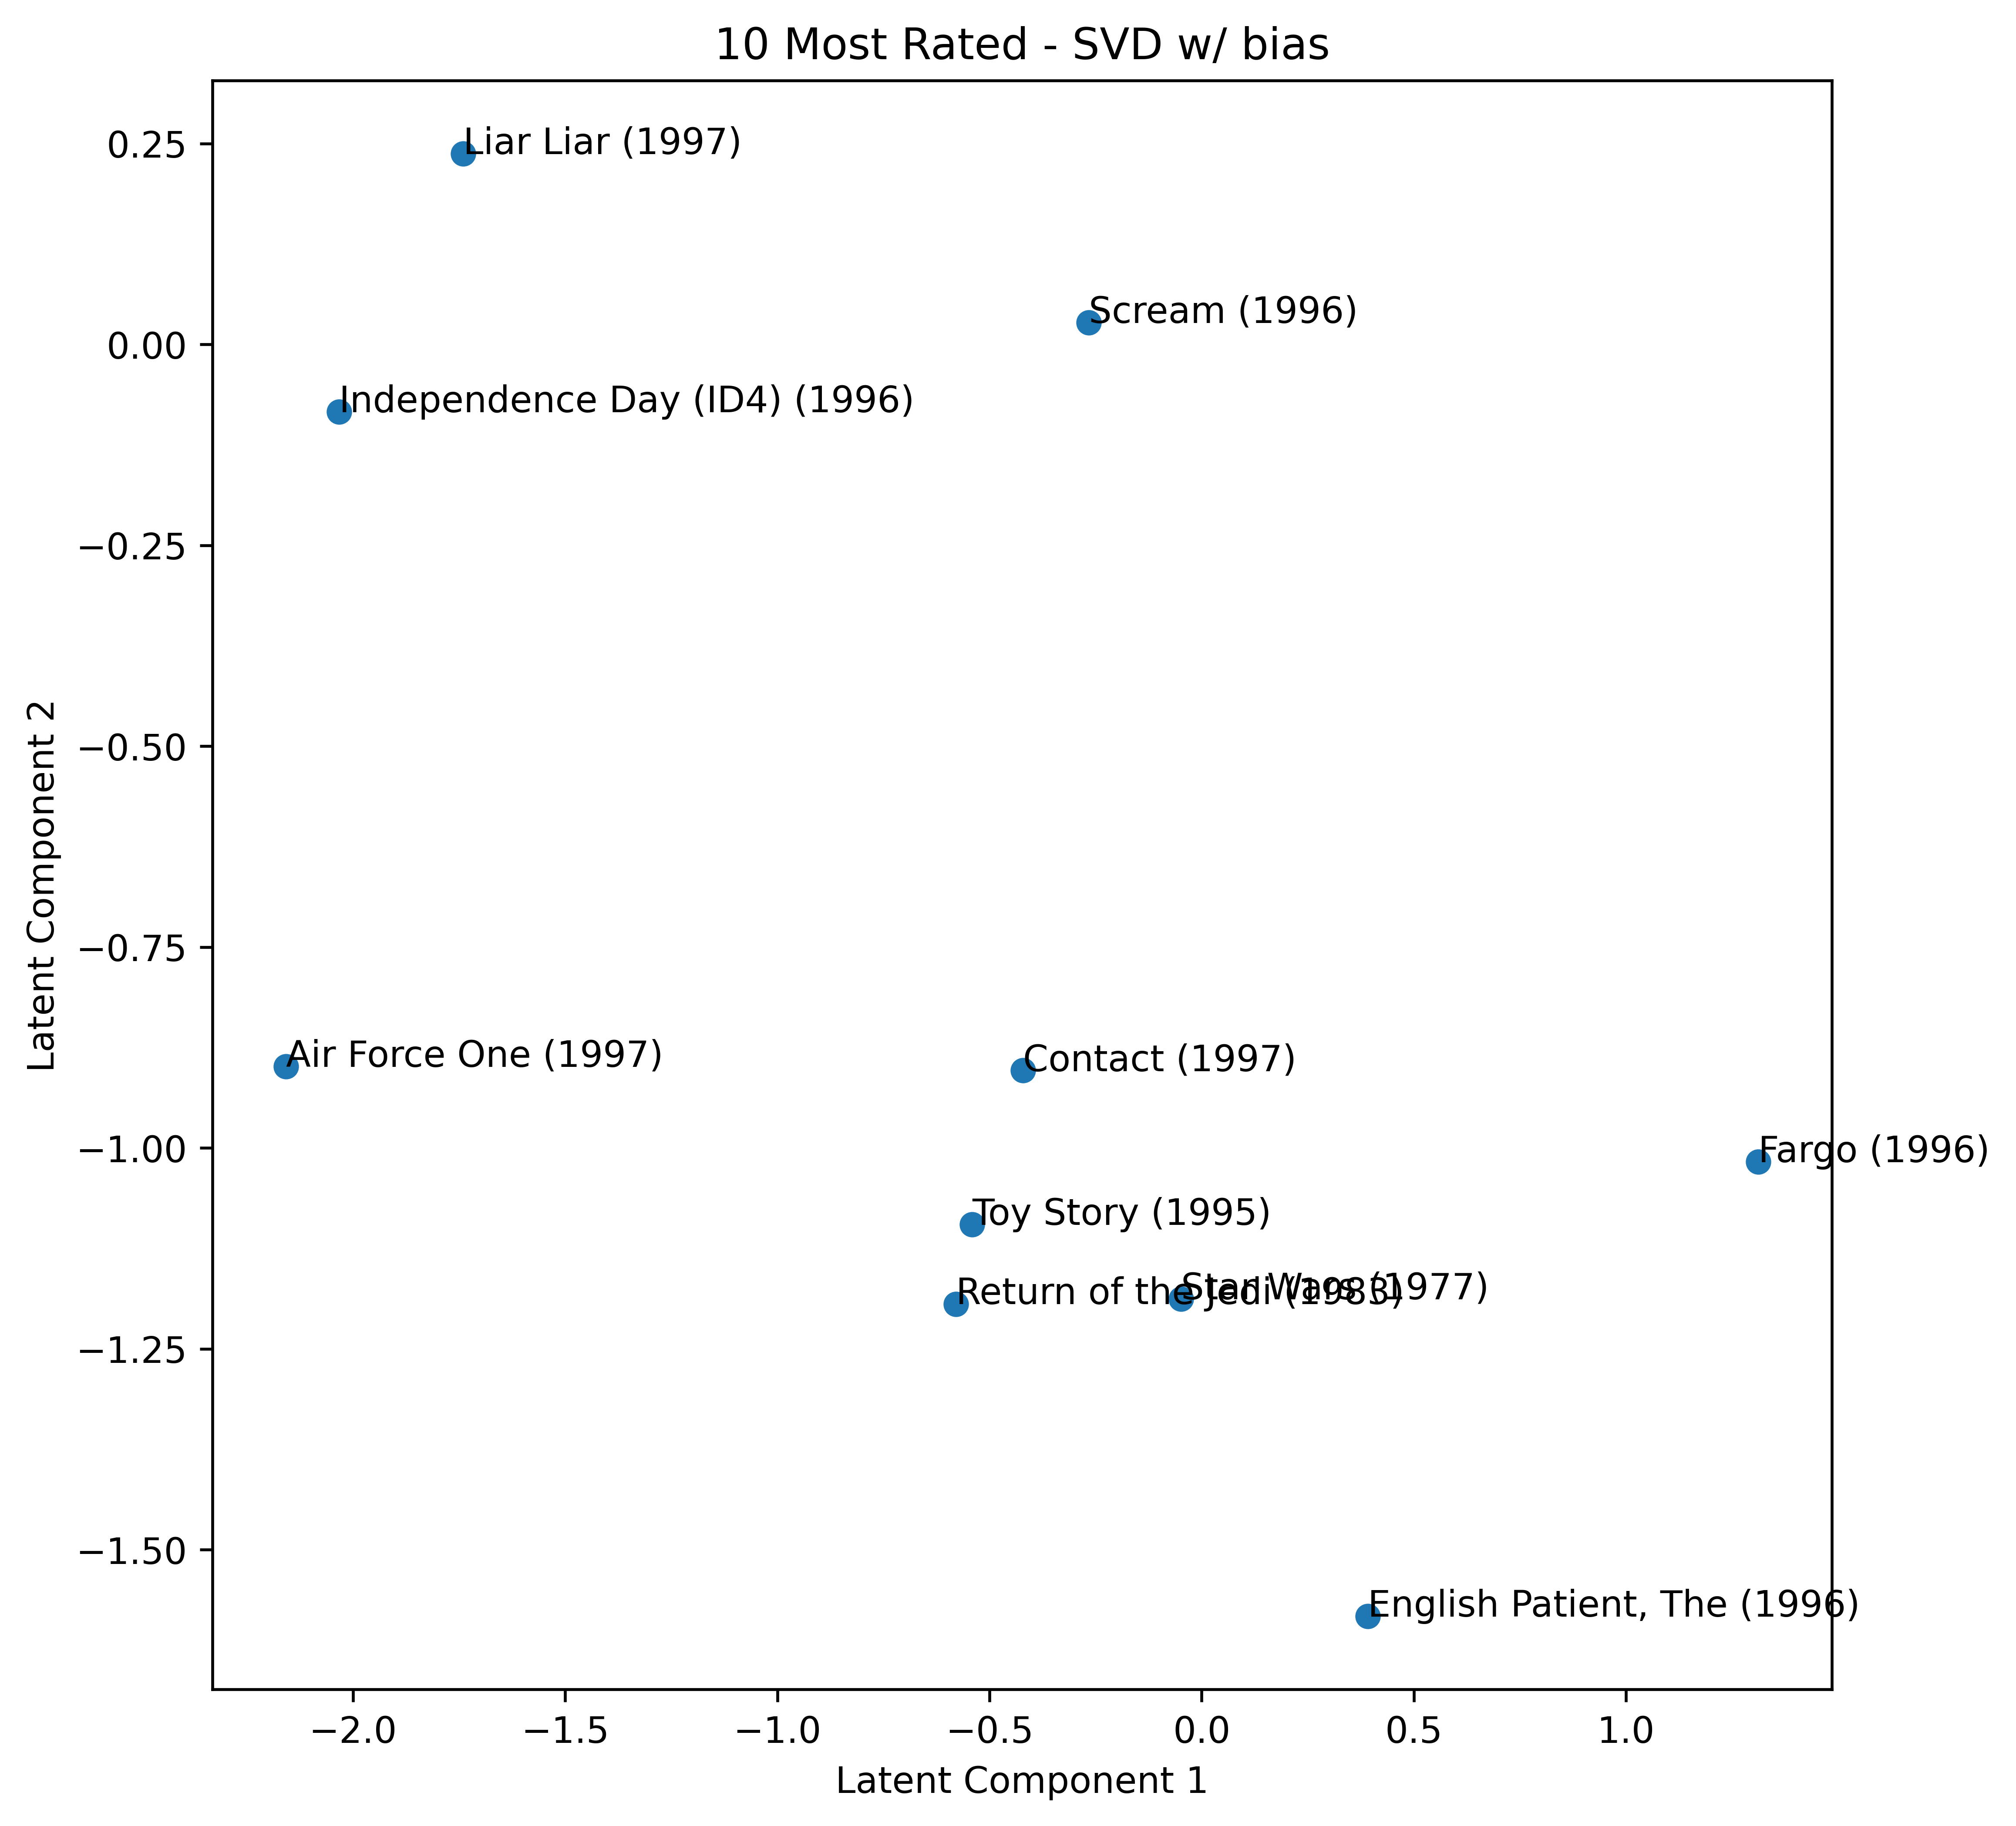
\includegraphics[width = 0.45\textwidth]{pop10_biased.png}}
\end{figure}
\begin{figure}[H]
    \centering 
    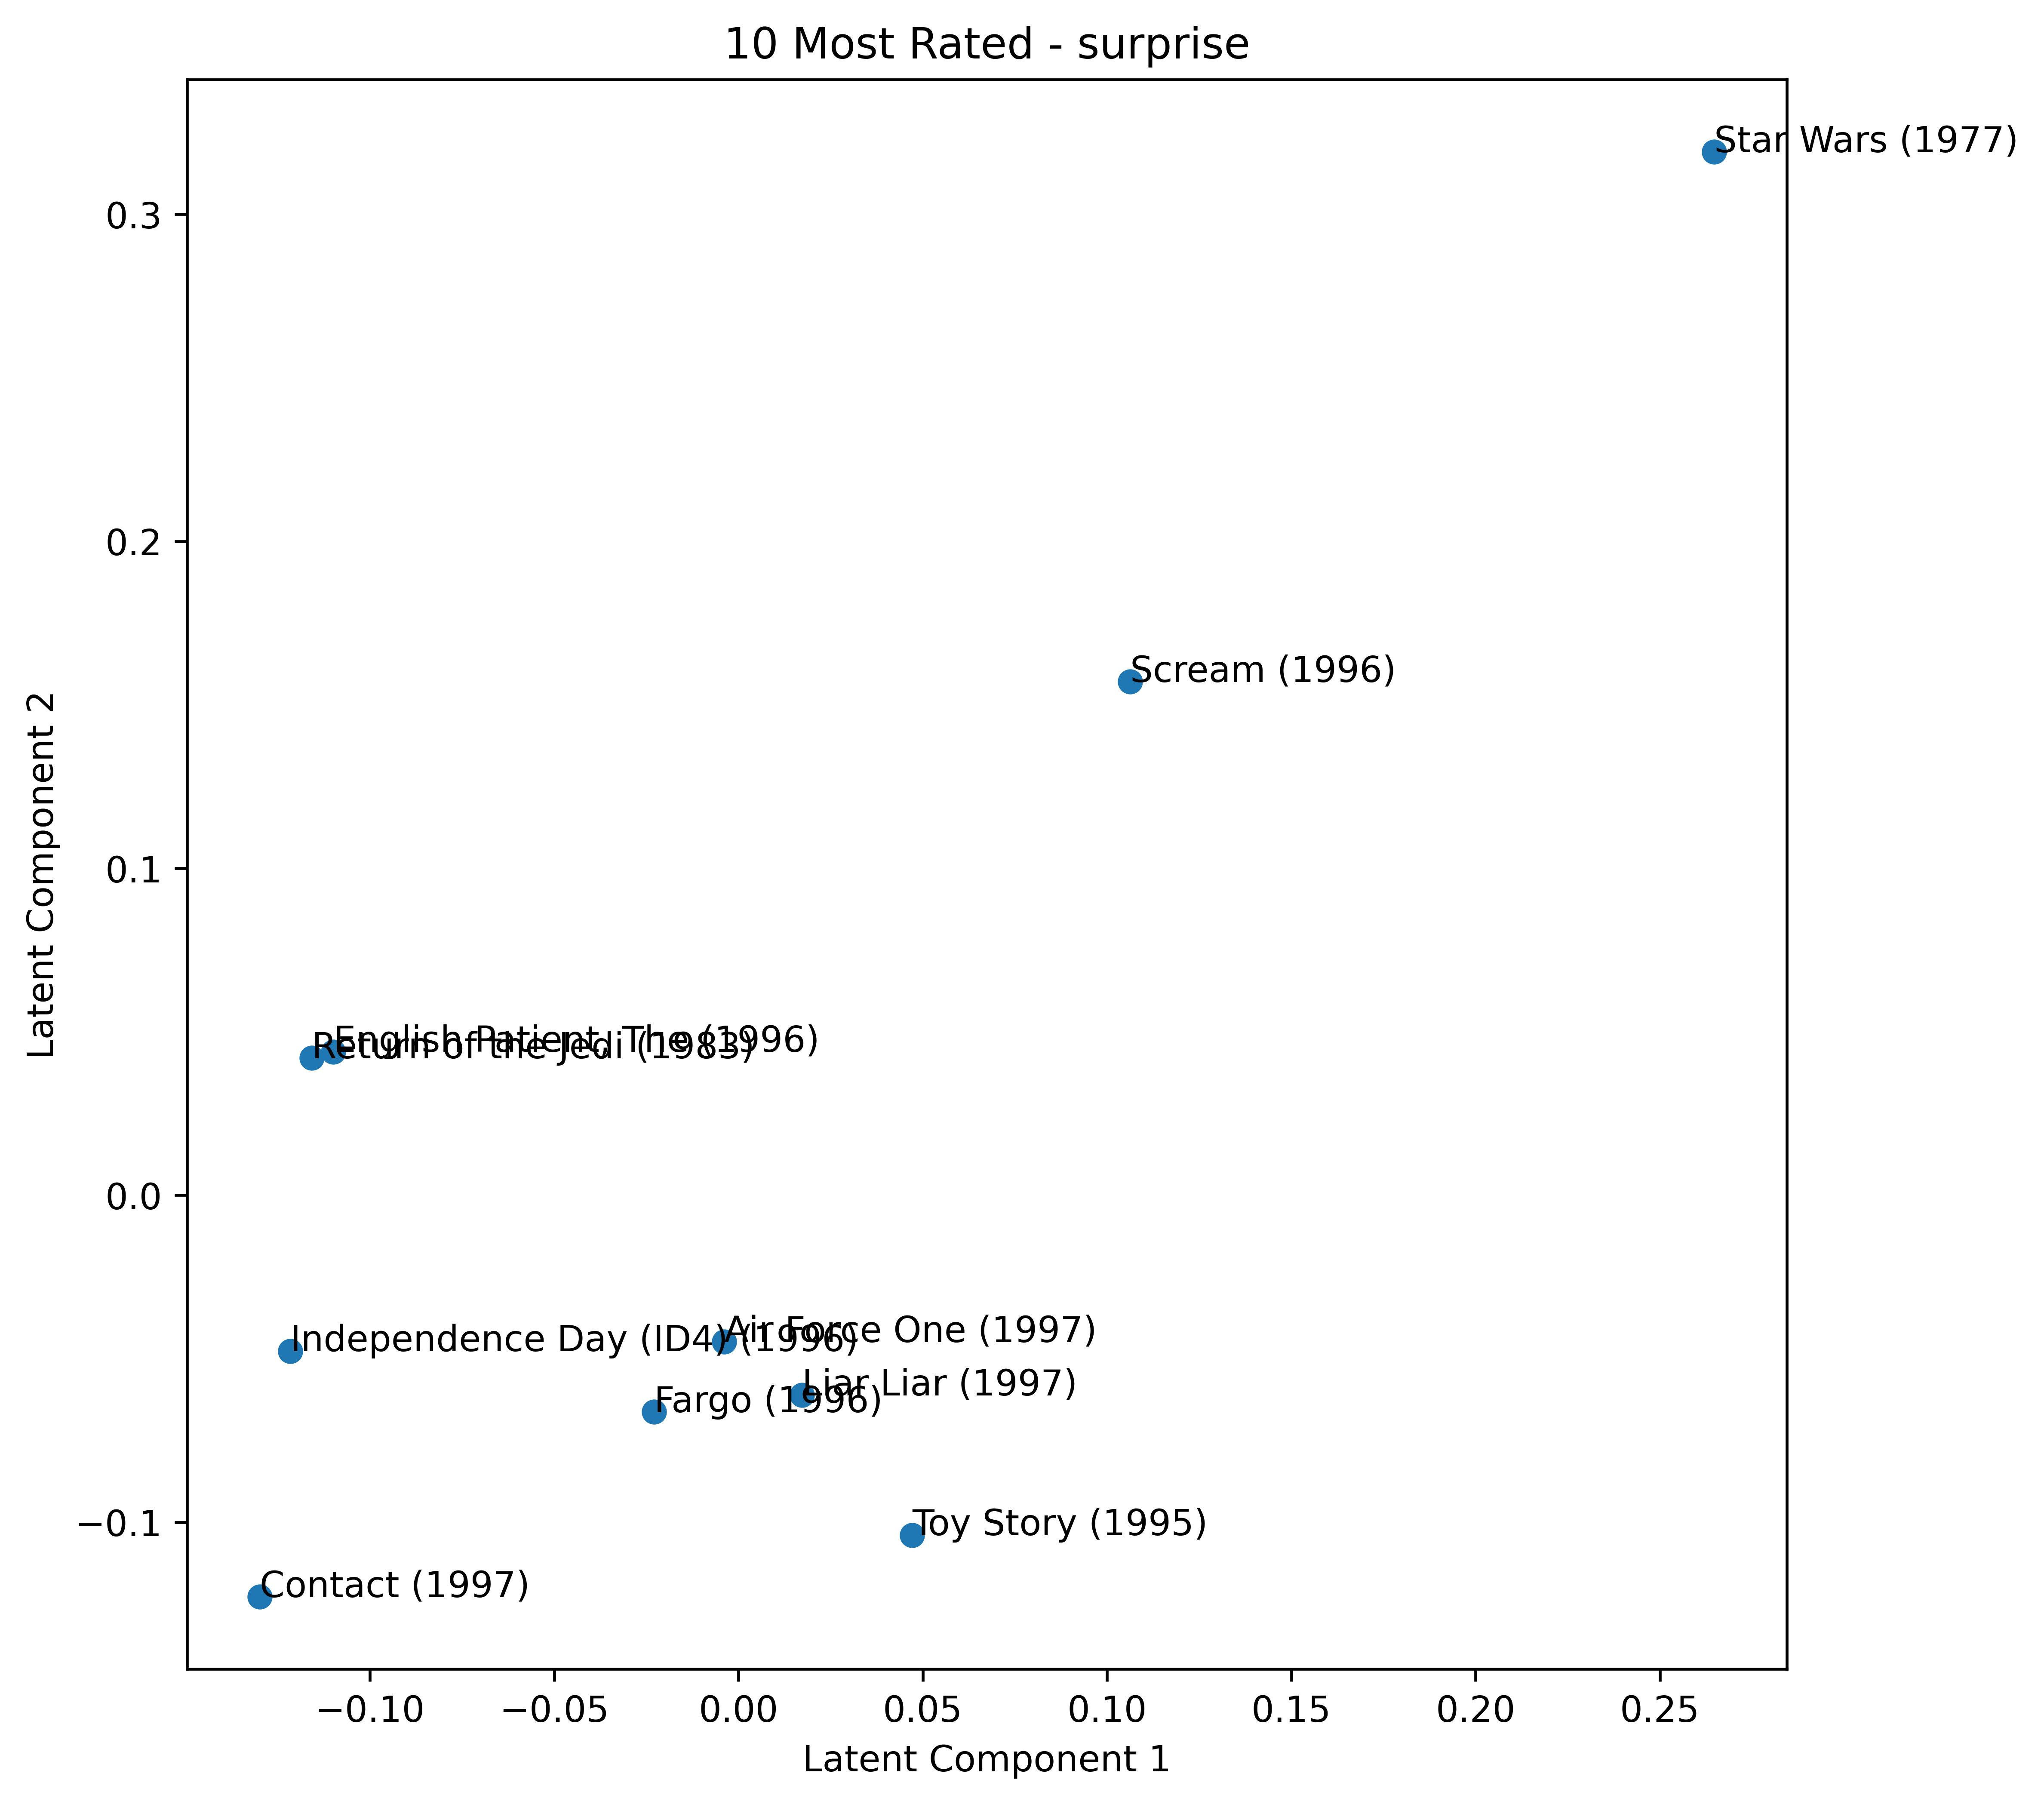
\includegraphics[width=7cm]{pop10_sp.png}
\end{figure}

The \texttt{surprise} implementatin of SVD does not appear to make as much use of the parameter space as either of the other two 
SVD implementations that we made. The placement of the different films does not make the most sense and it surely reflected of the 
subpar performance that \texttt{surprise} yielded on the test set.
\par 
When looking at the our own SVD implementations, most movies have been shifted around by a decent amount but largely remain in the same 
quadrants as they had been in previously. \textit{Air Force One} and \textit{The English Patient} had the greatest shifts with \textit{Air 
Force One} moving to an entirely new quadrant, but otherwise most points remain roughly in place. Some of the positions of these points make 
sense, for instance the two Star Wars films being close to each other in both plots. Meanwhile other point positions seem more questionable, 
such as \textit{Independence Day} and \textit{Contact} not being near each other despite both being sci-fi films.

\subsection{Horror movies}

\begin{figure}[H]
    \centering
    \subfloat{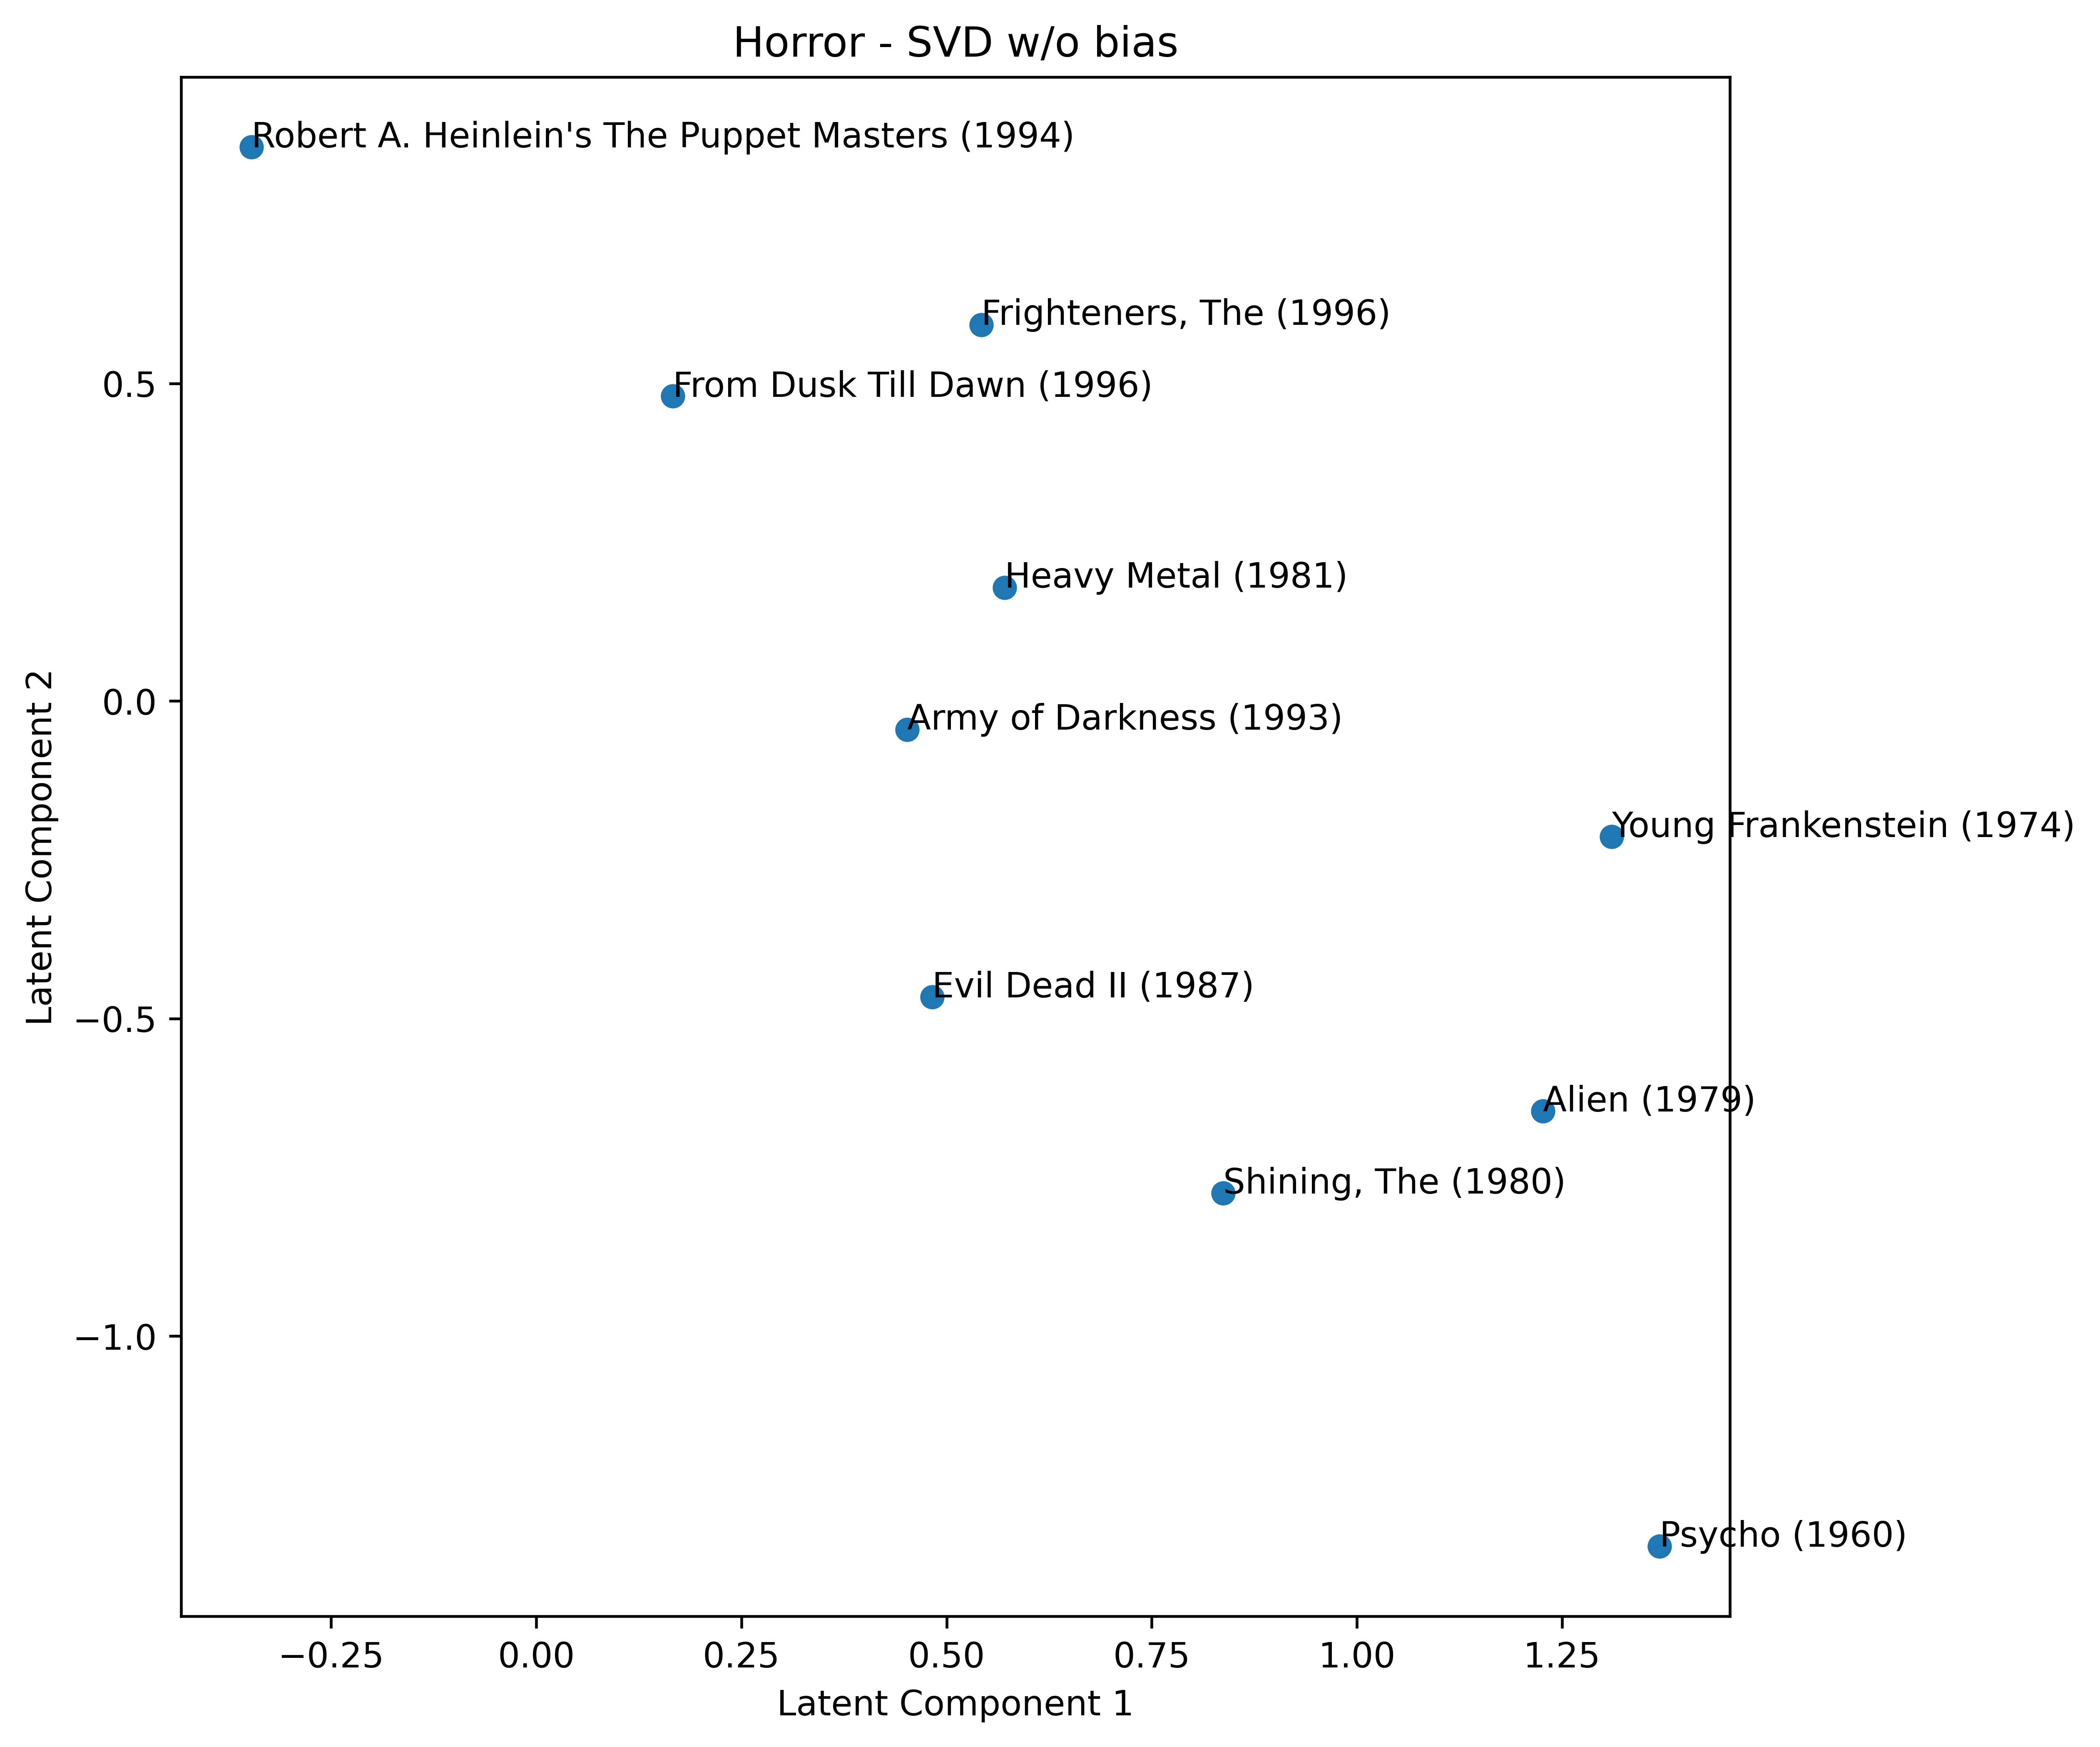
\includegraphics[width = 0.45\textwidth]{horror_SVD.png}}
    \subfloat{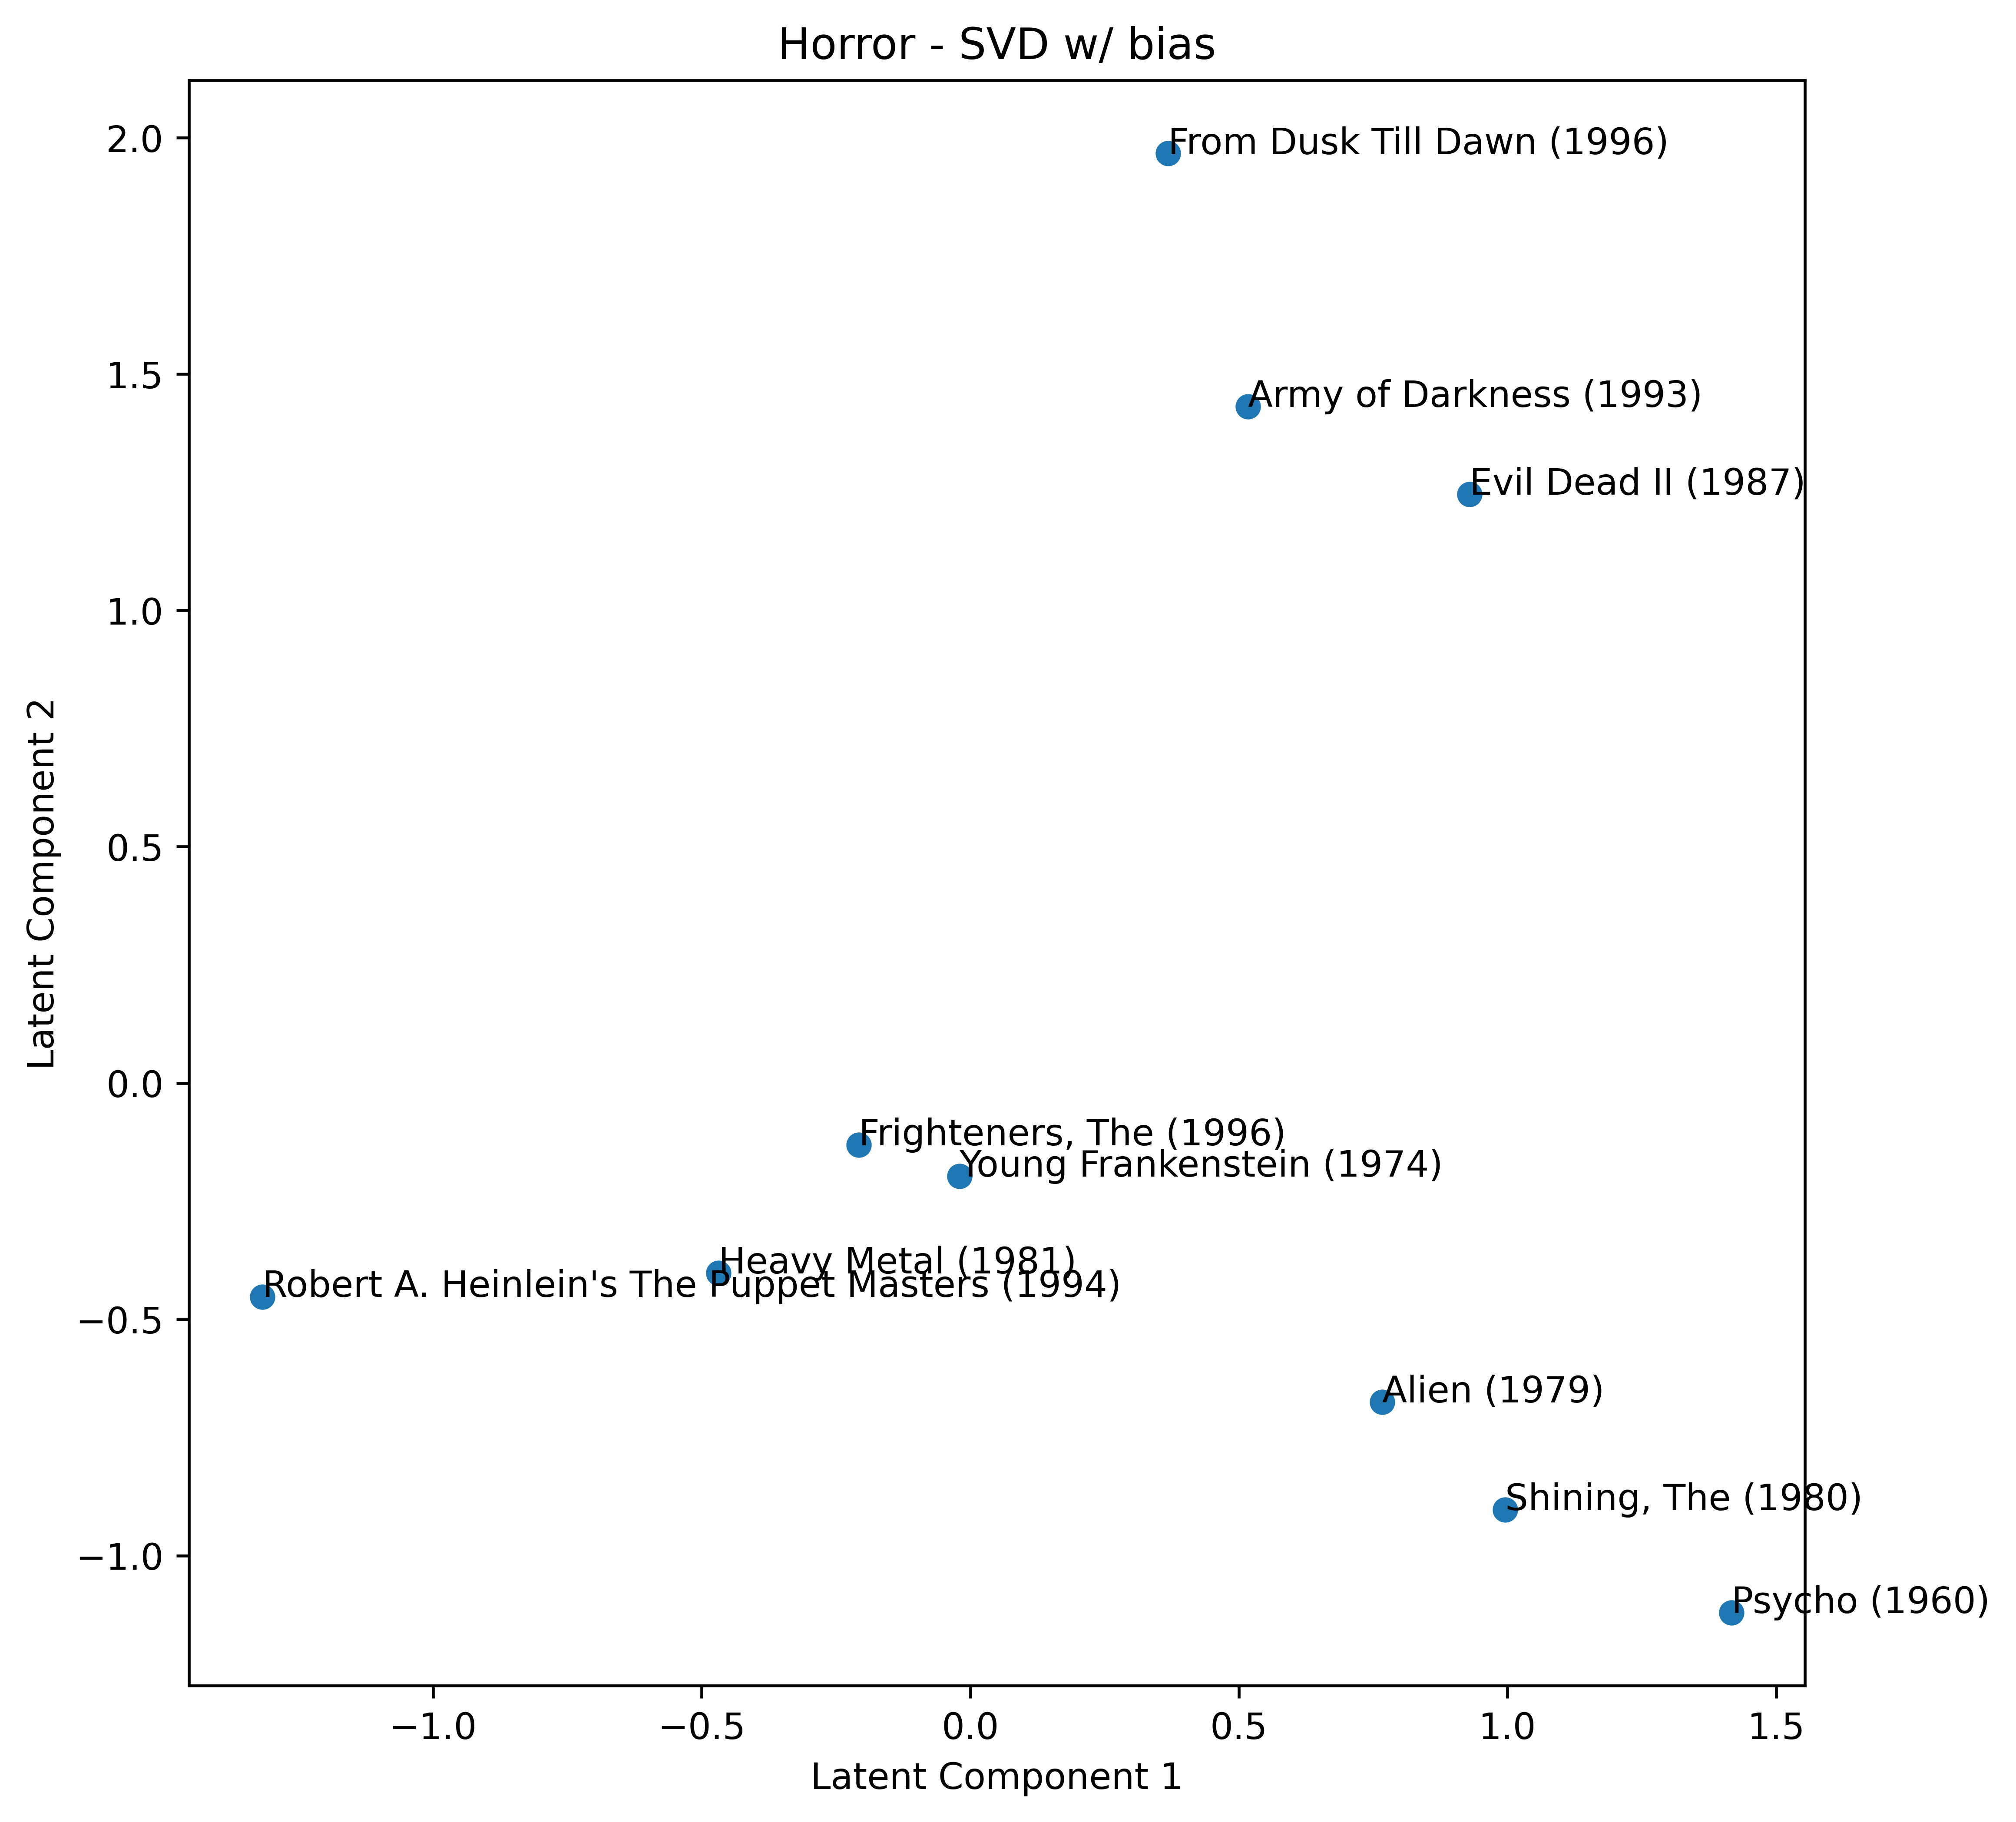
\includegraphics[width = 0.45\textwidth]{horror_SVD_biased.png}}
\end{figure}
\begin{figure}[H]
    \centering 
    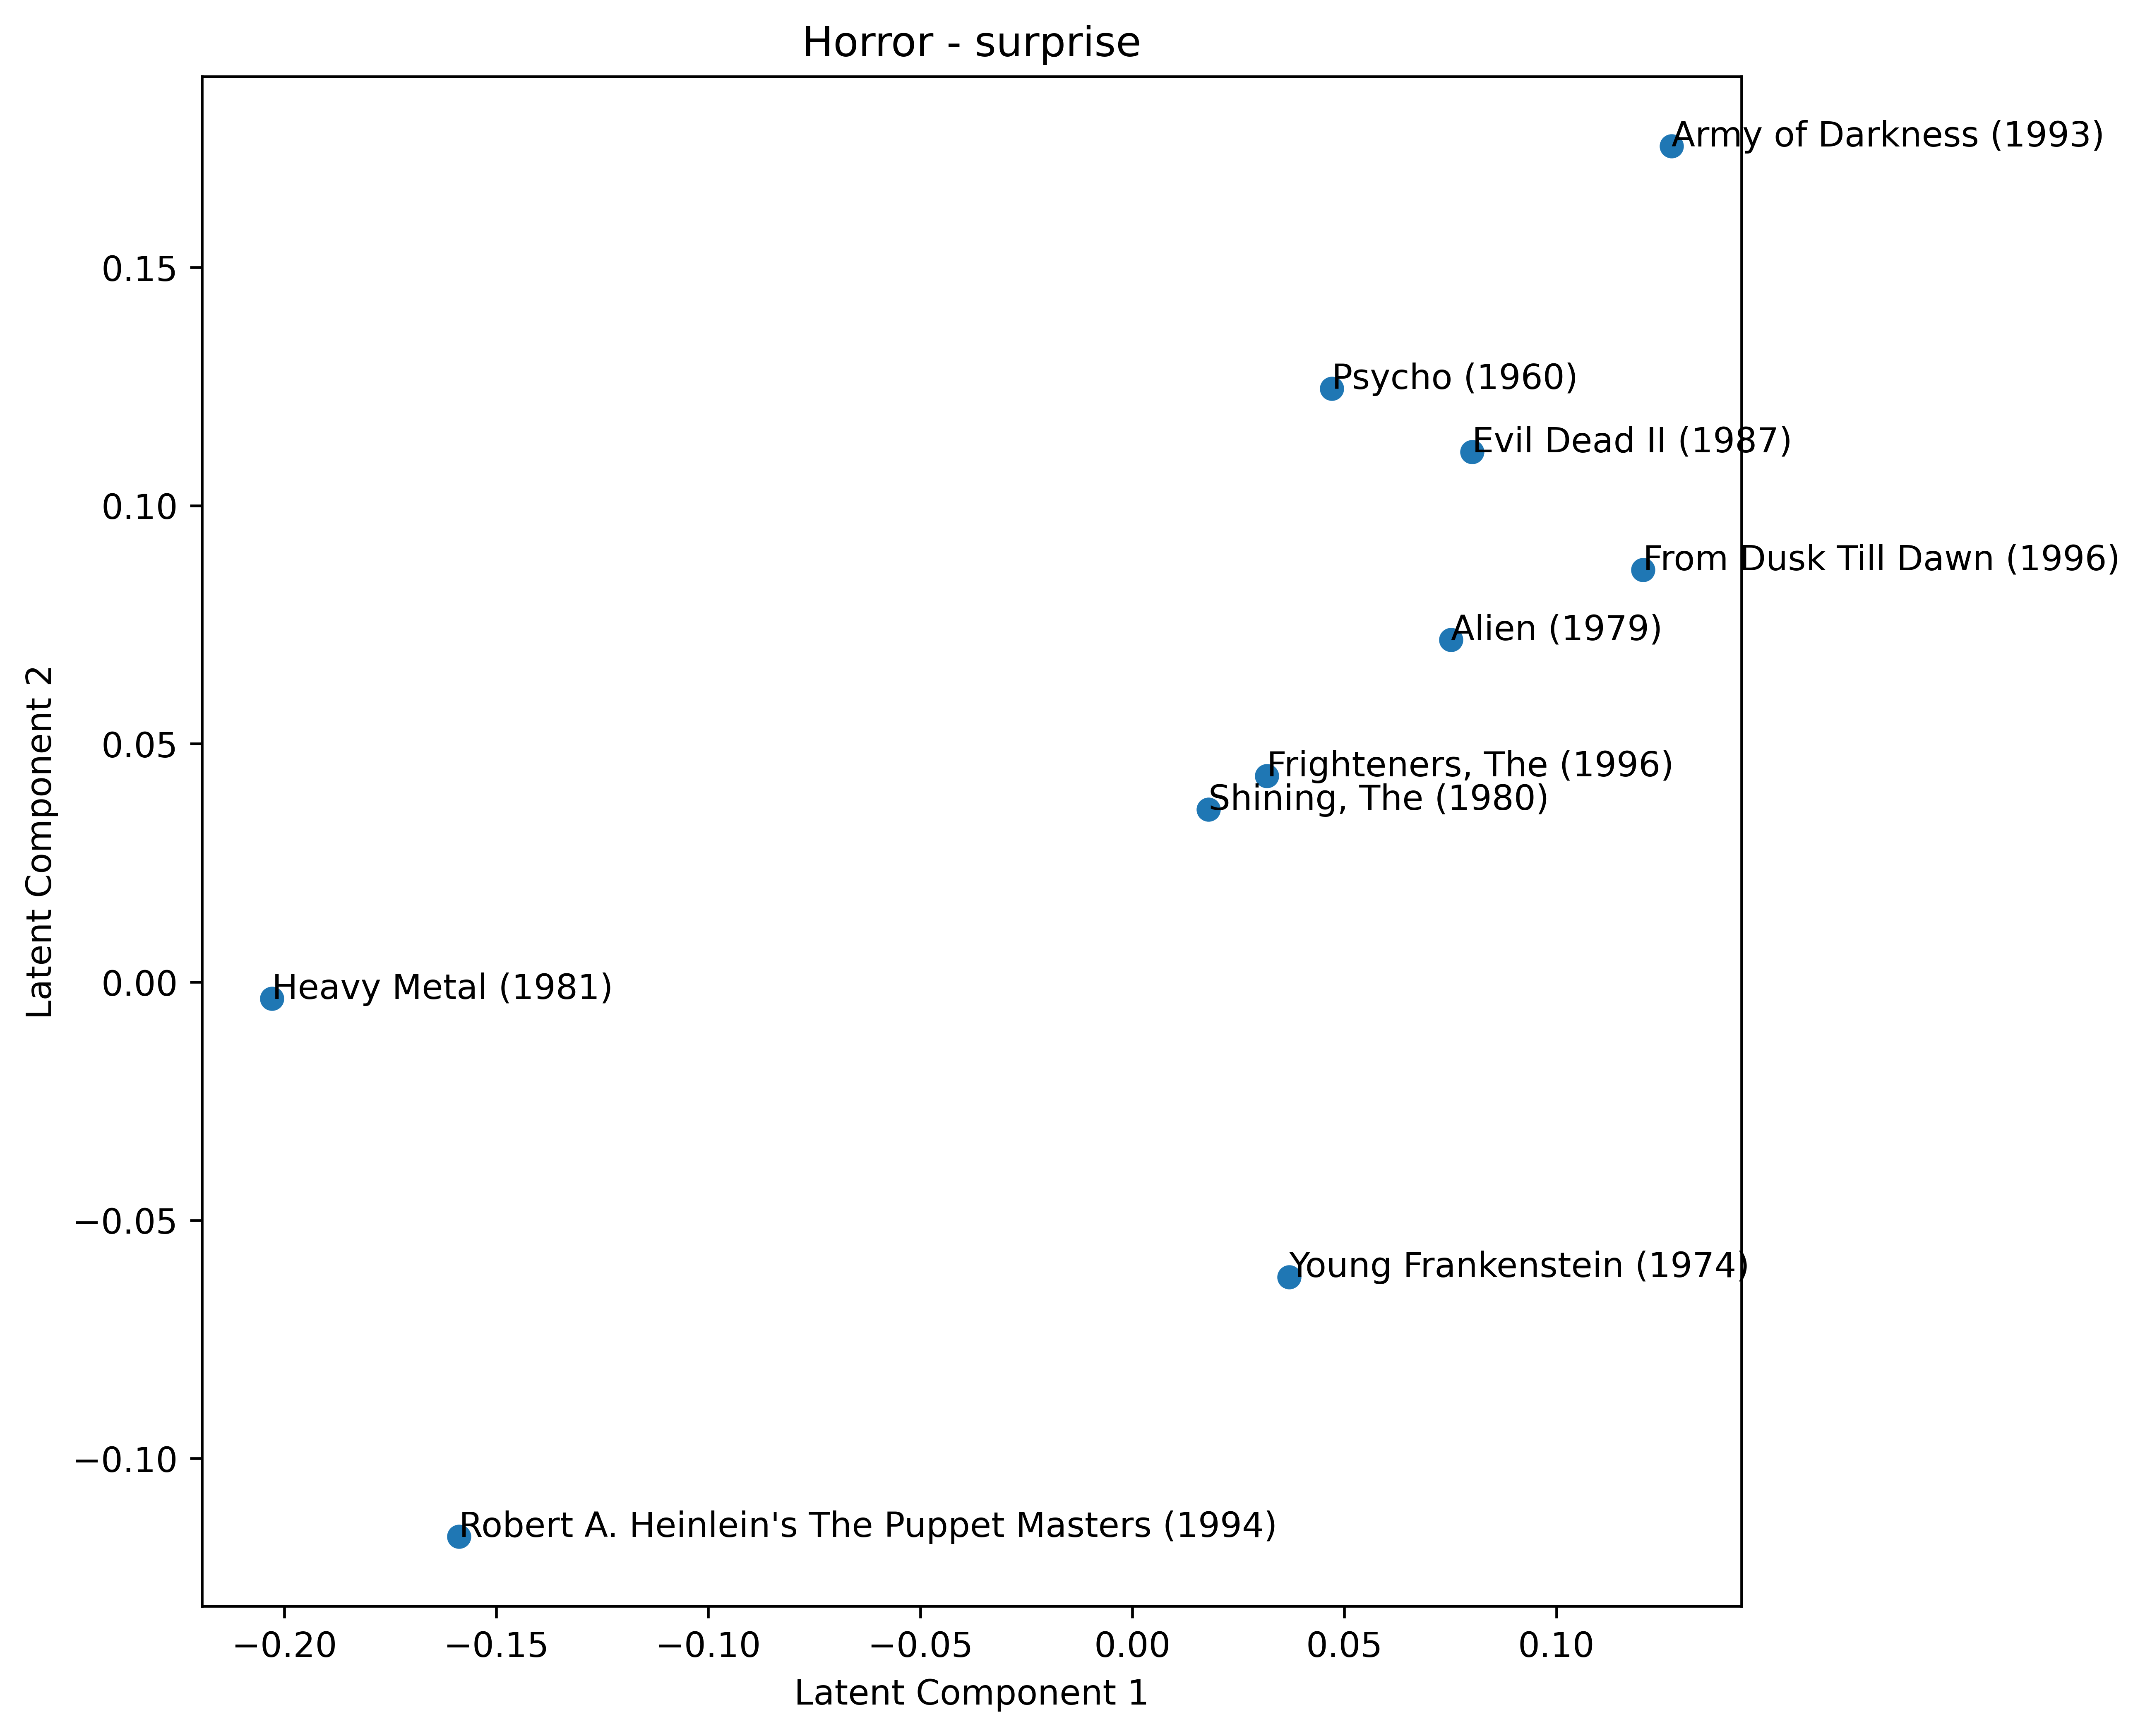
\includegraphics[width=10cm]{horror_SVD_sp.png}
\end{figure}

The horror films appear to be subject to more clustering than the other film groups we've looked at. The \texttt{surprise} implementation is most 
guilty of this and does not appear to make a clear distinction between different subgenres of horror. The top right quadrant of our plot 
puts together horror films with comedic, mystery, and action elements together.
\par 
The other two SVD implementations seem to do a better job at clustering cimilar movies. For instance, we would expect \textit{The Shining} and 
\textit{Psycho} to be near each other on the basis that they are both horror/mystery thrillers. \textit{Alien}, also being in the horror/mystery 
category is located near these other two movies. \textit{Army of Darkness} and \textit{Evil Dead II} are also near each other in both plots 
as horror/comedy films. The remaining films don't seem to be scattered too coherently. Interestingly, the SVD model without the bias terms 
displays these points as a diagonal continuum across the parameter space while the SVD model with the bias terms is more willing to cluster 
movies in an isolated fashion.

\subsection{Crime movies}

\begin{figure}[H]
    \centering
    \subfloat{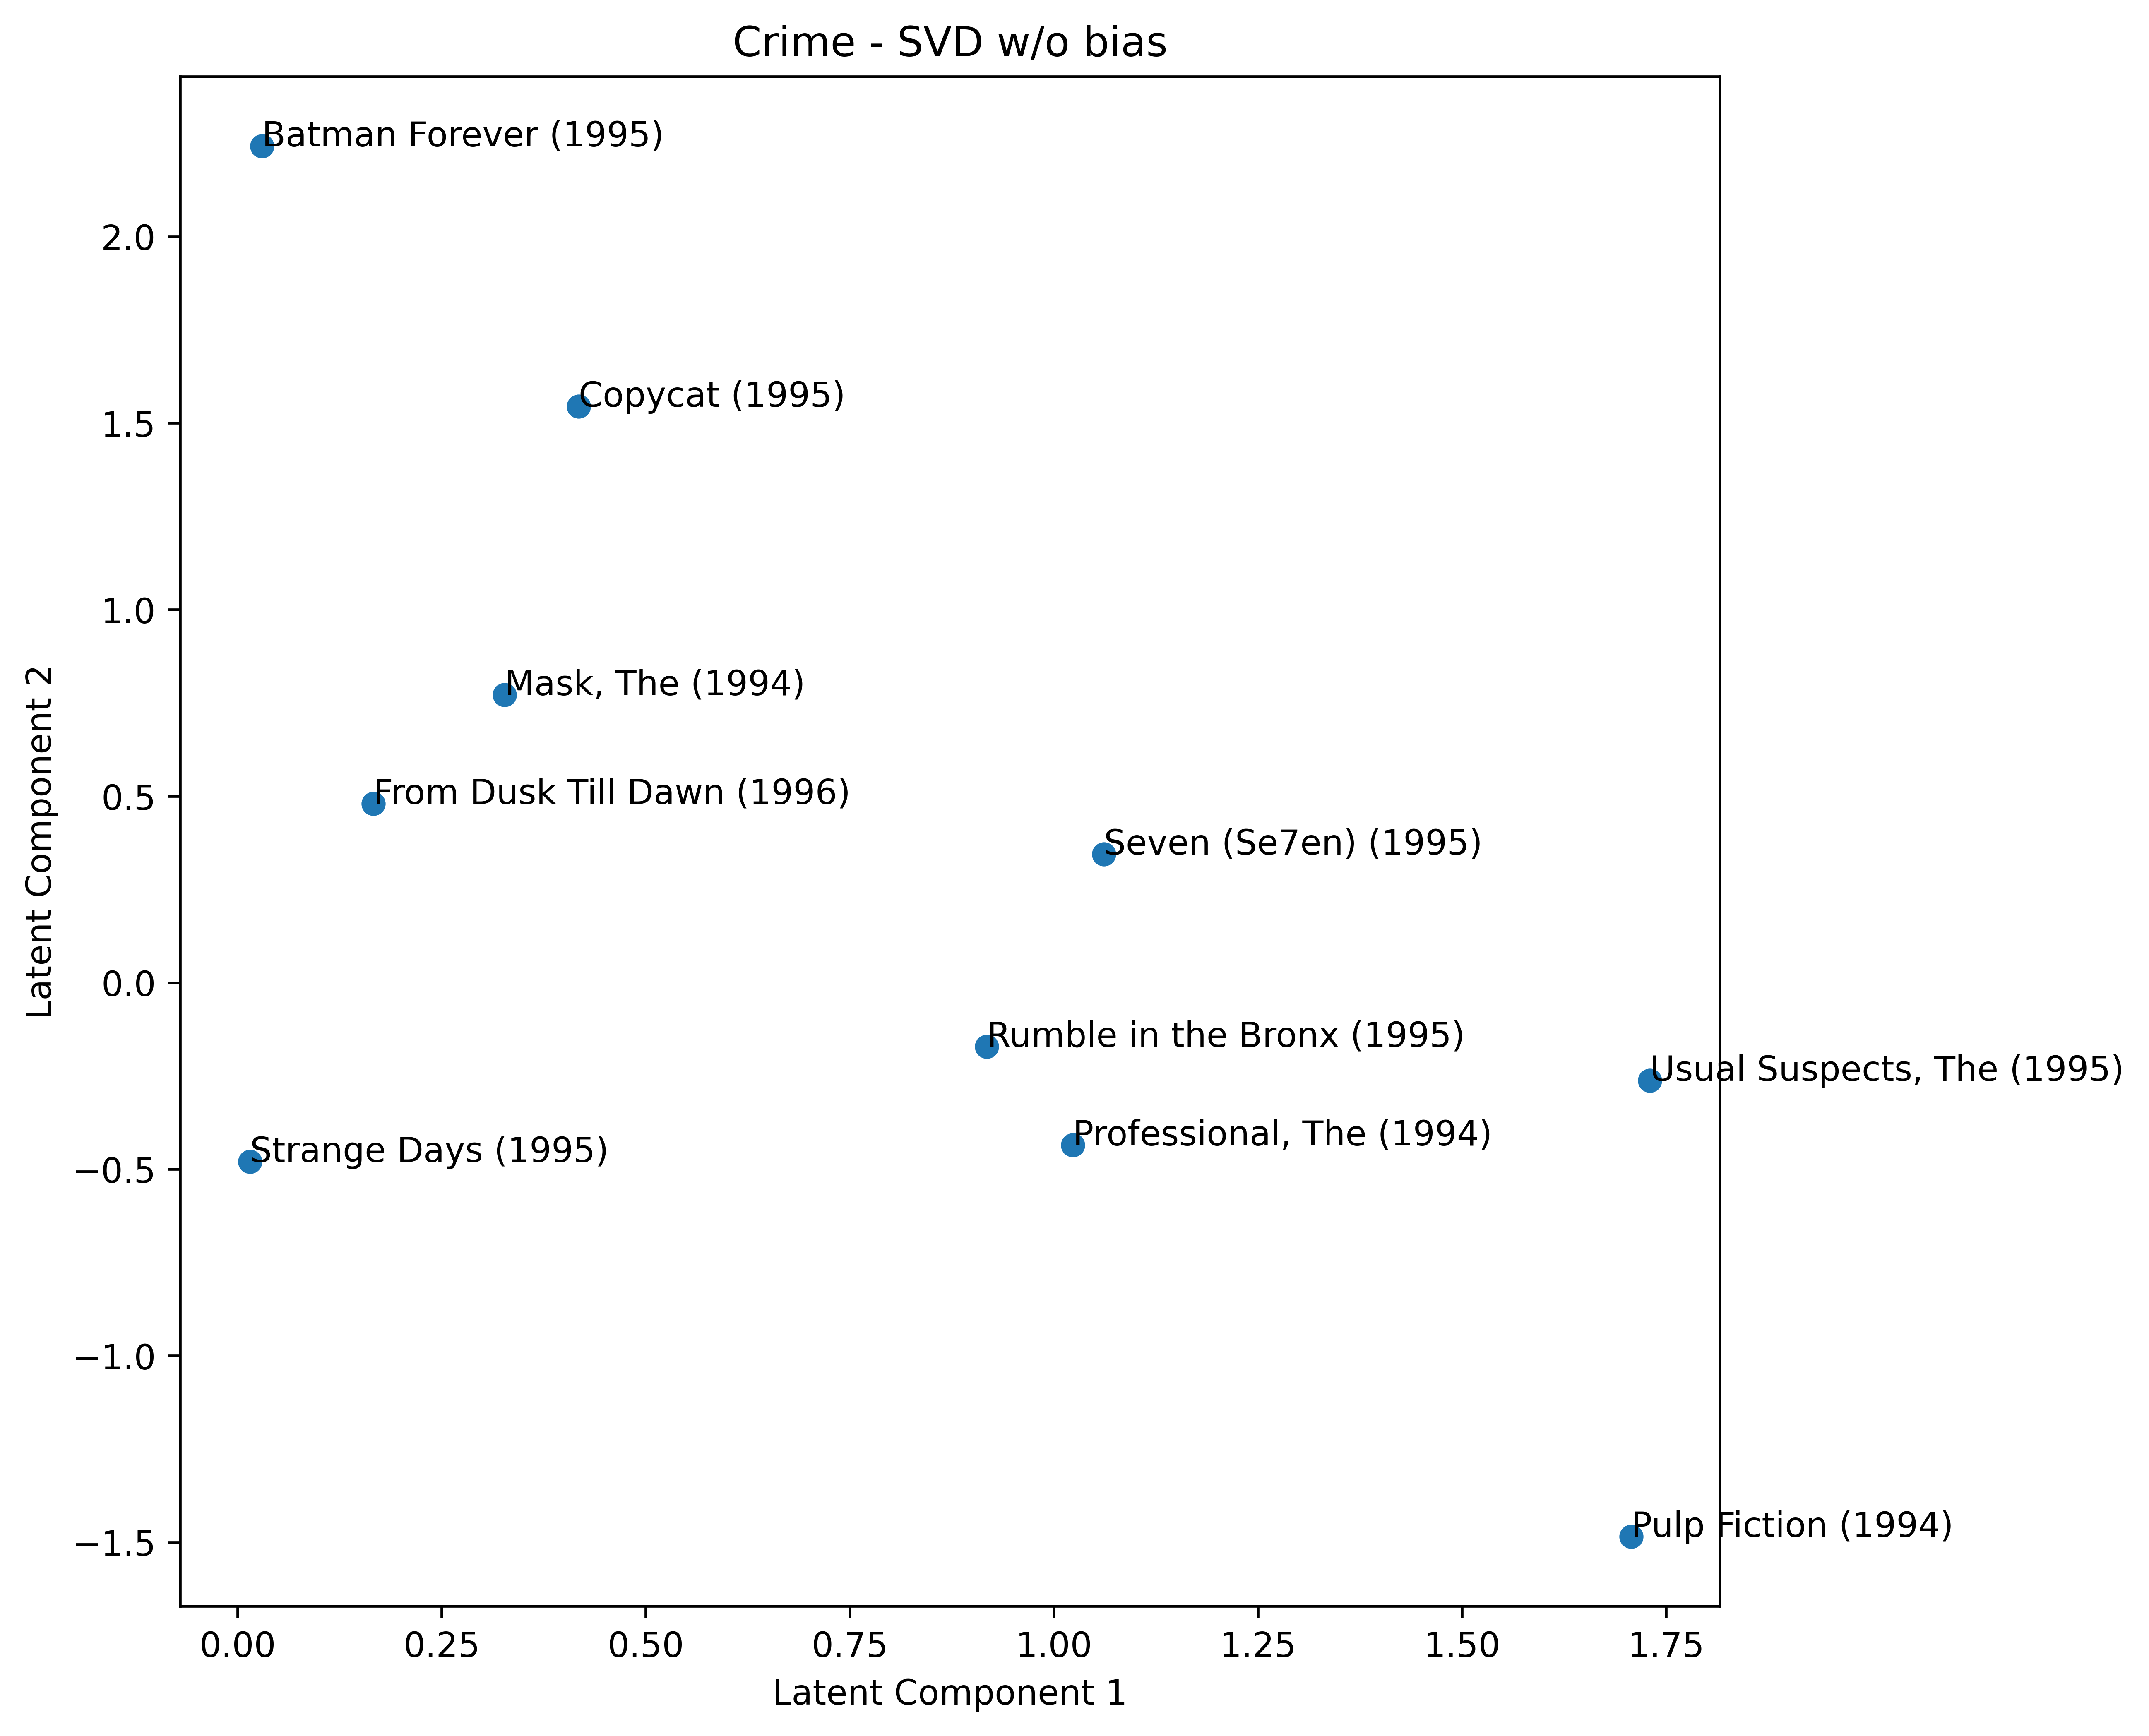
\includegraphics[width = 0.45\textwidth]{crime_SVD.png}}
    \subfloat{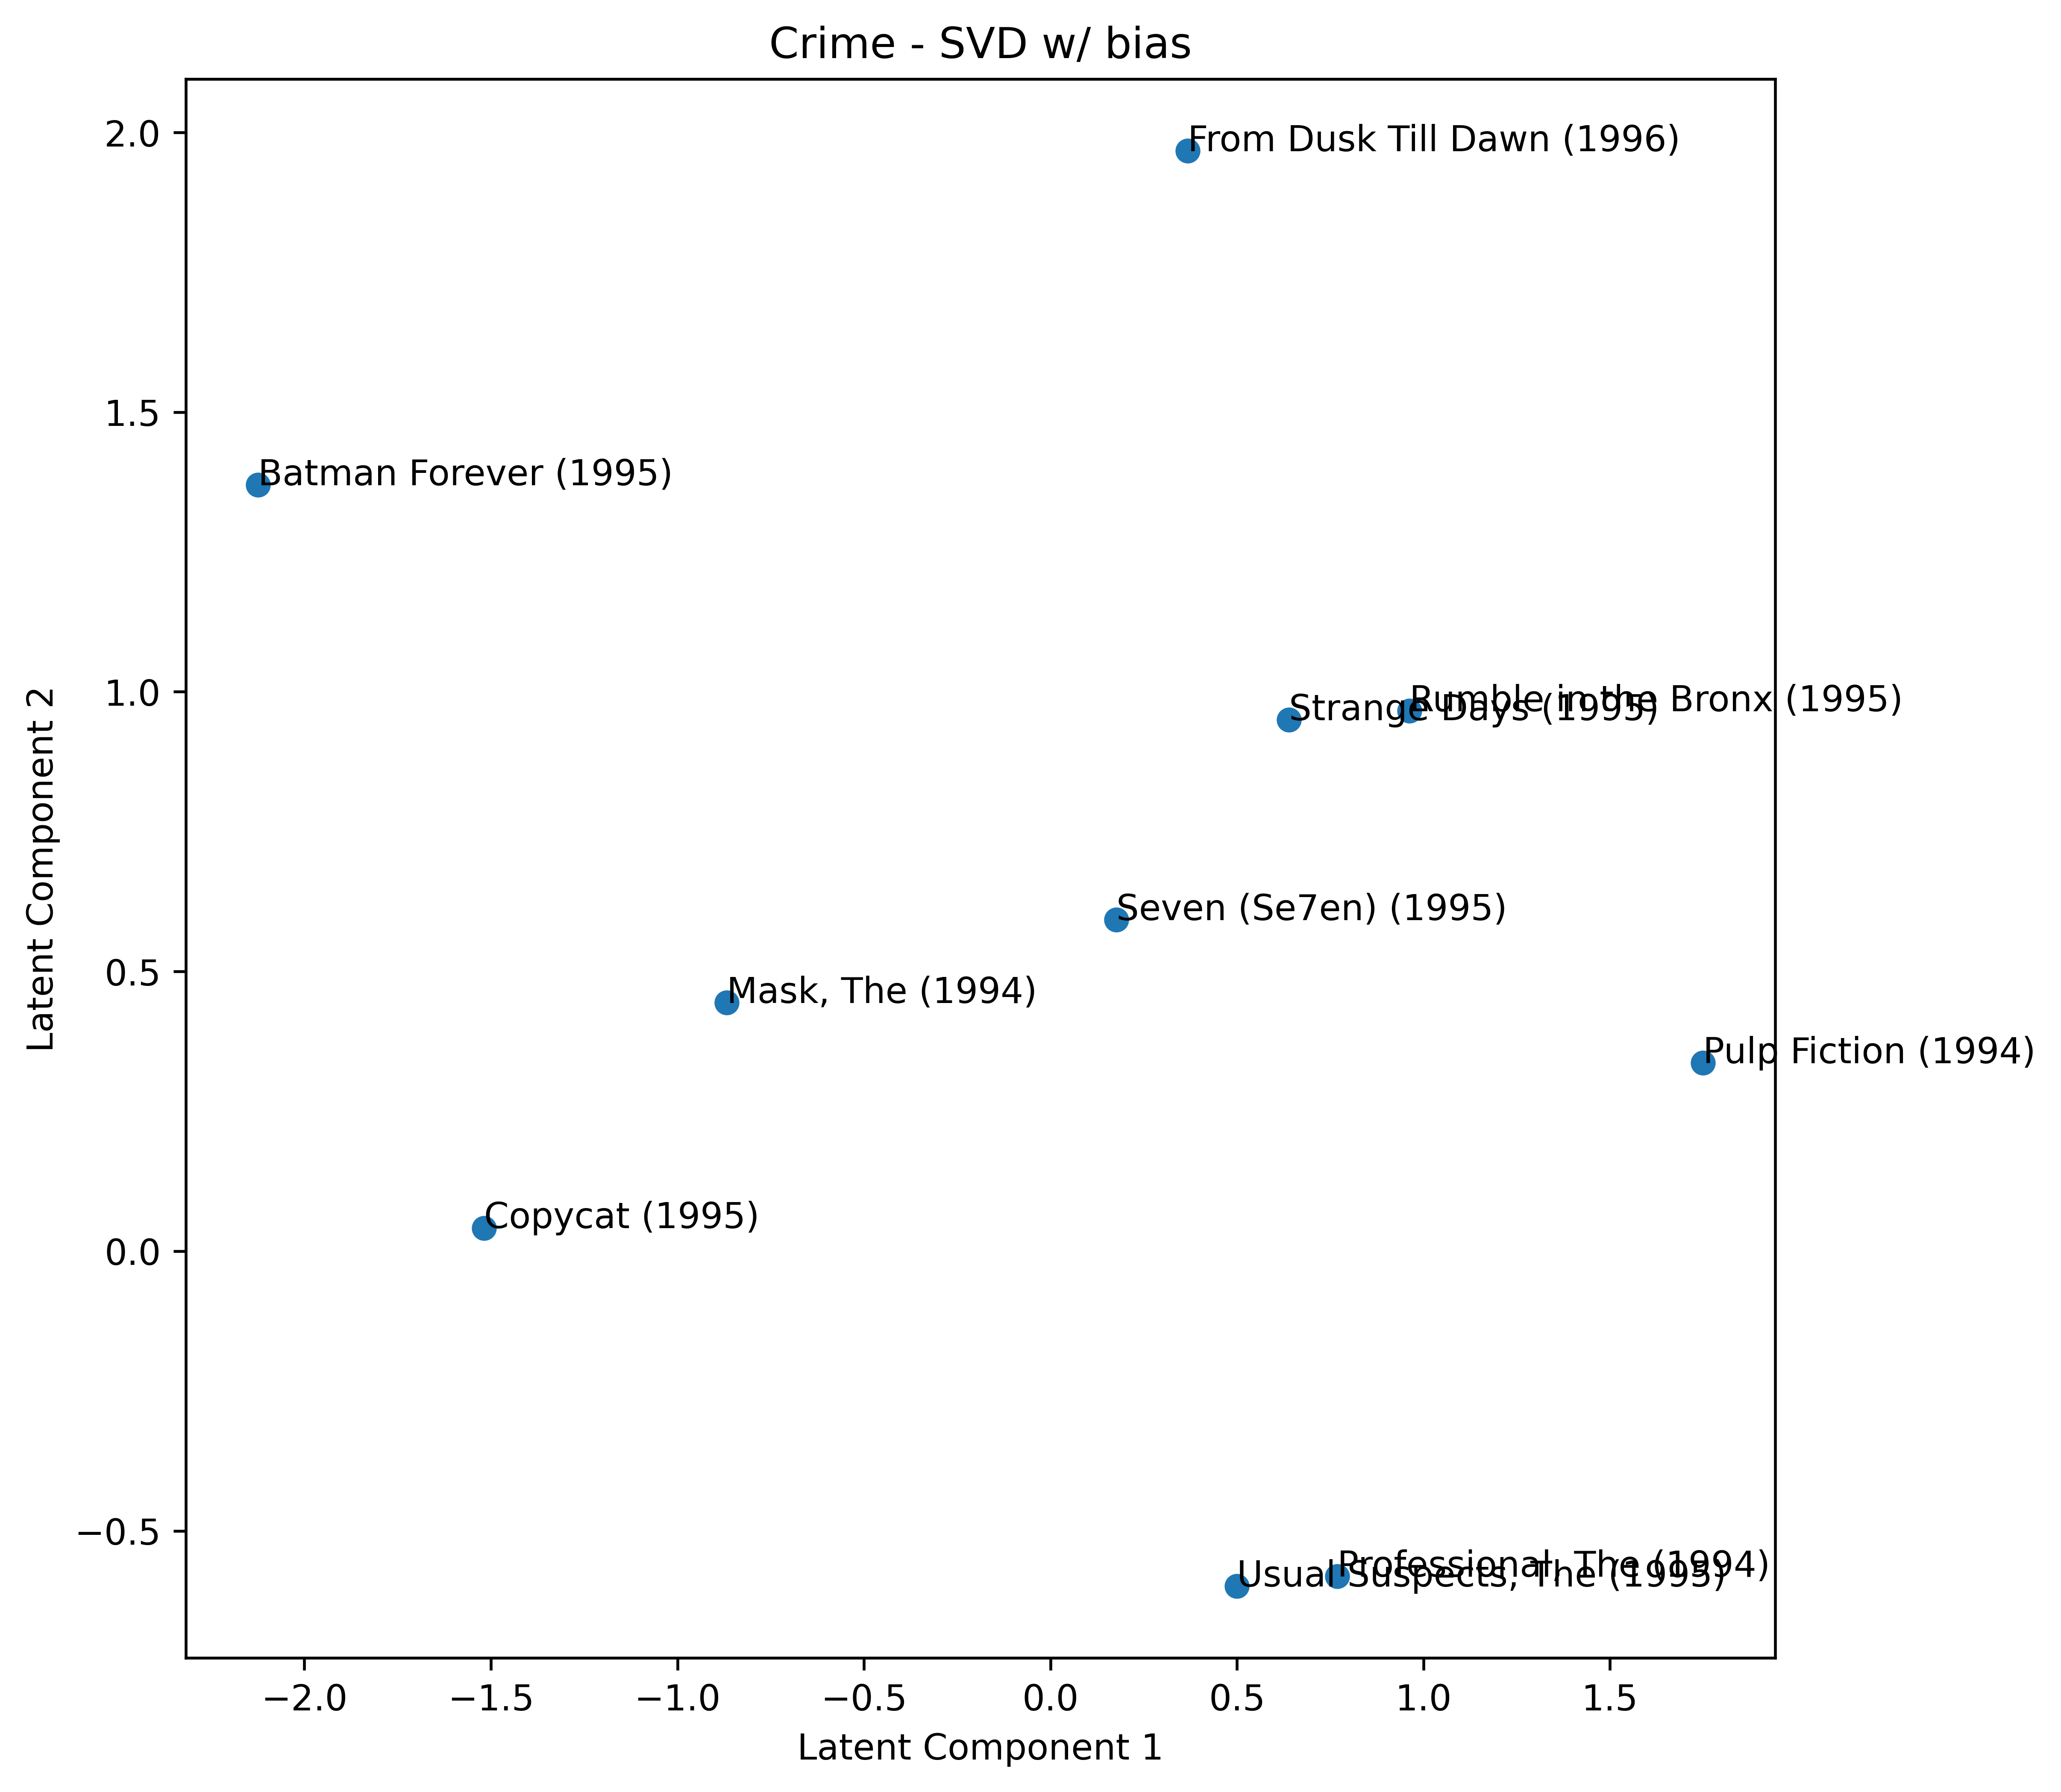
\includegraphics[width = 0.45\textwidth]{crime_SVD_biased.png}}
\end{figure}
\begin{figure}[H]
    \centering 
    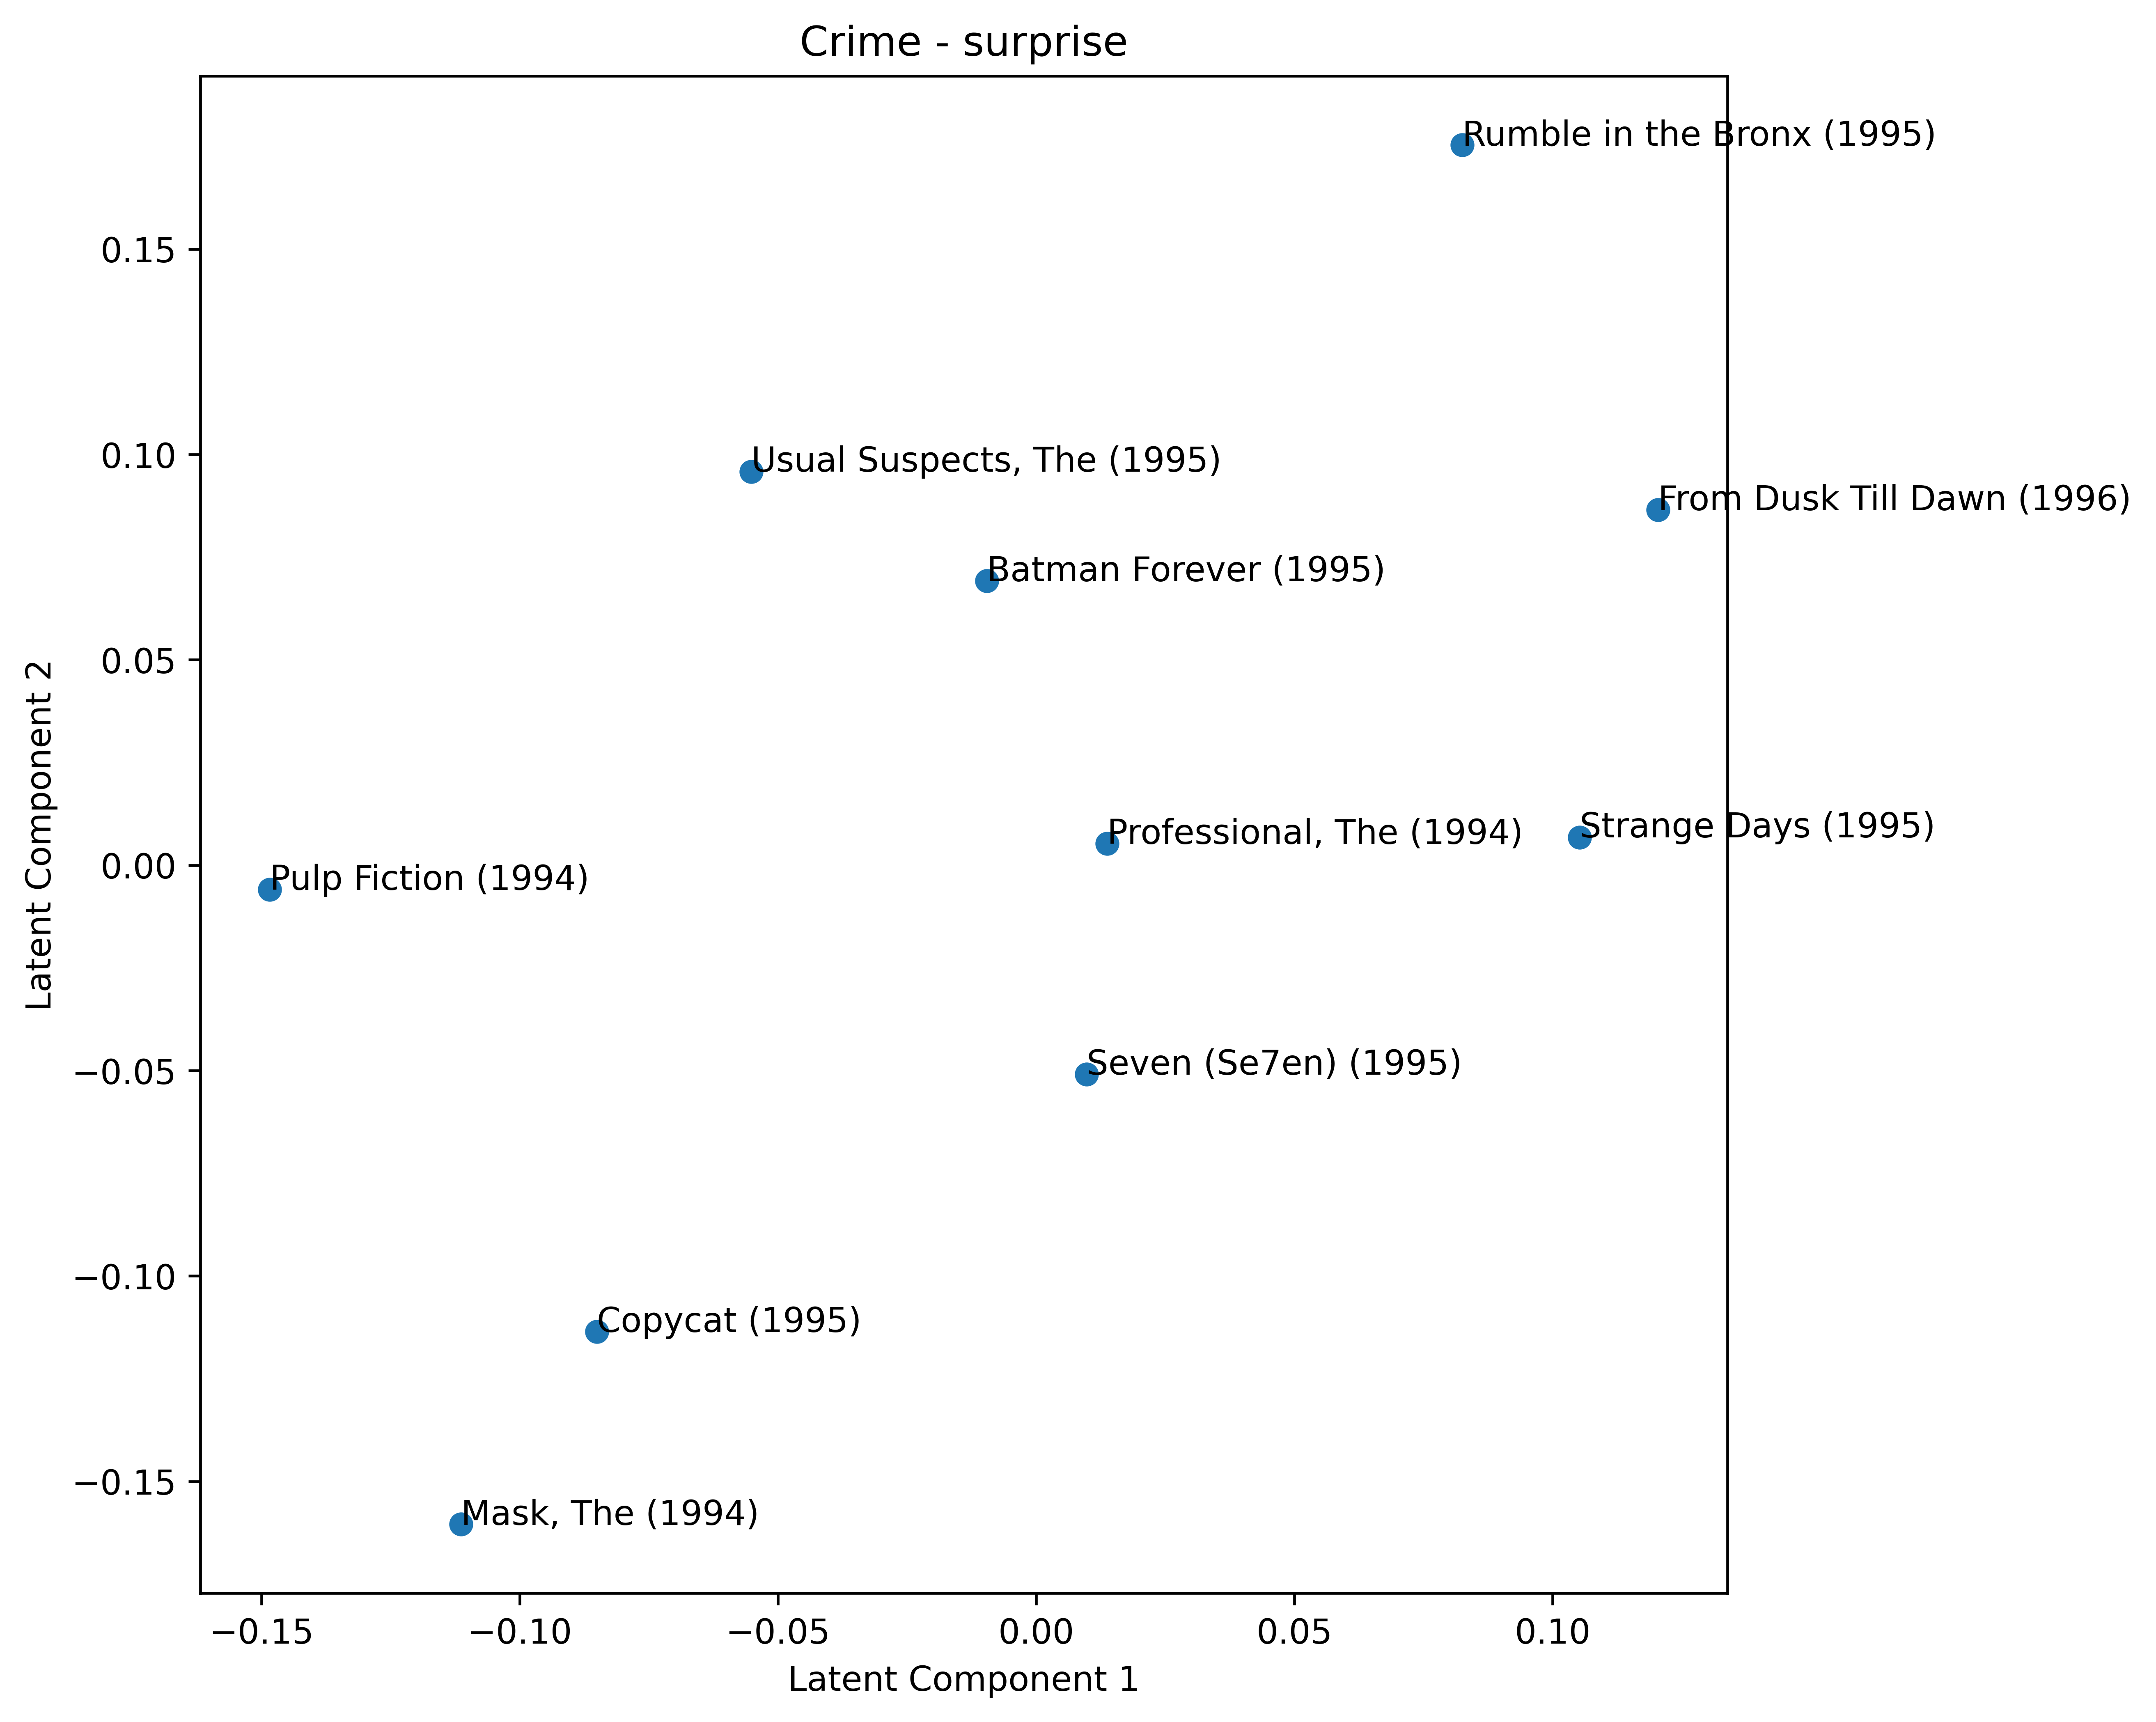
\includegraphics[width=10cm]{crime_SVD_sp.png}
\end{figure}

All of our models seemed to struggle with the crime movies than any other the other sets of films, though some trends are common among them. 
\textit{Pulp Fiction} manages to be somewhat of an outlier in every plot, maybe due to its relative popularity compared to the other films 
that are being included. \textit{The Profession} and \textit{The Usual Suspects} are close to each other in every plot, though none of the other 
really seem to have similar clustering tendencies. There are three comedy/crime films: \textit{Batman Forever}, \textit{The Mask}, and \textit{
Rumble in the Bronx}, none of which seem to group up in any plot.

\subsection{Western movies}

\begin{figure}[H]
    \centering
    \subfloat{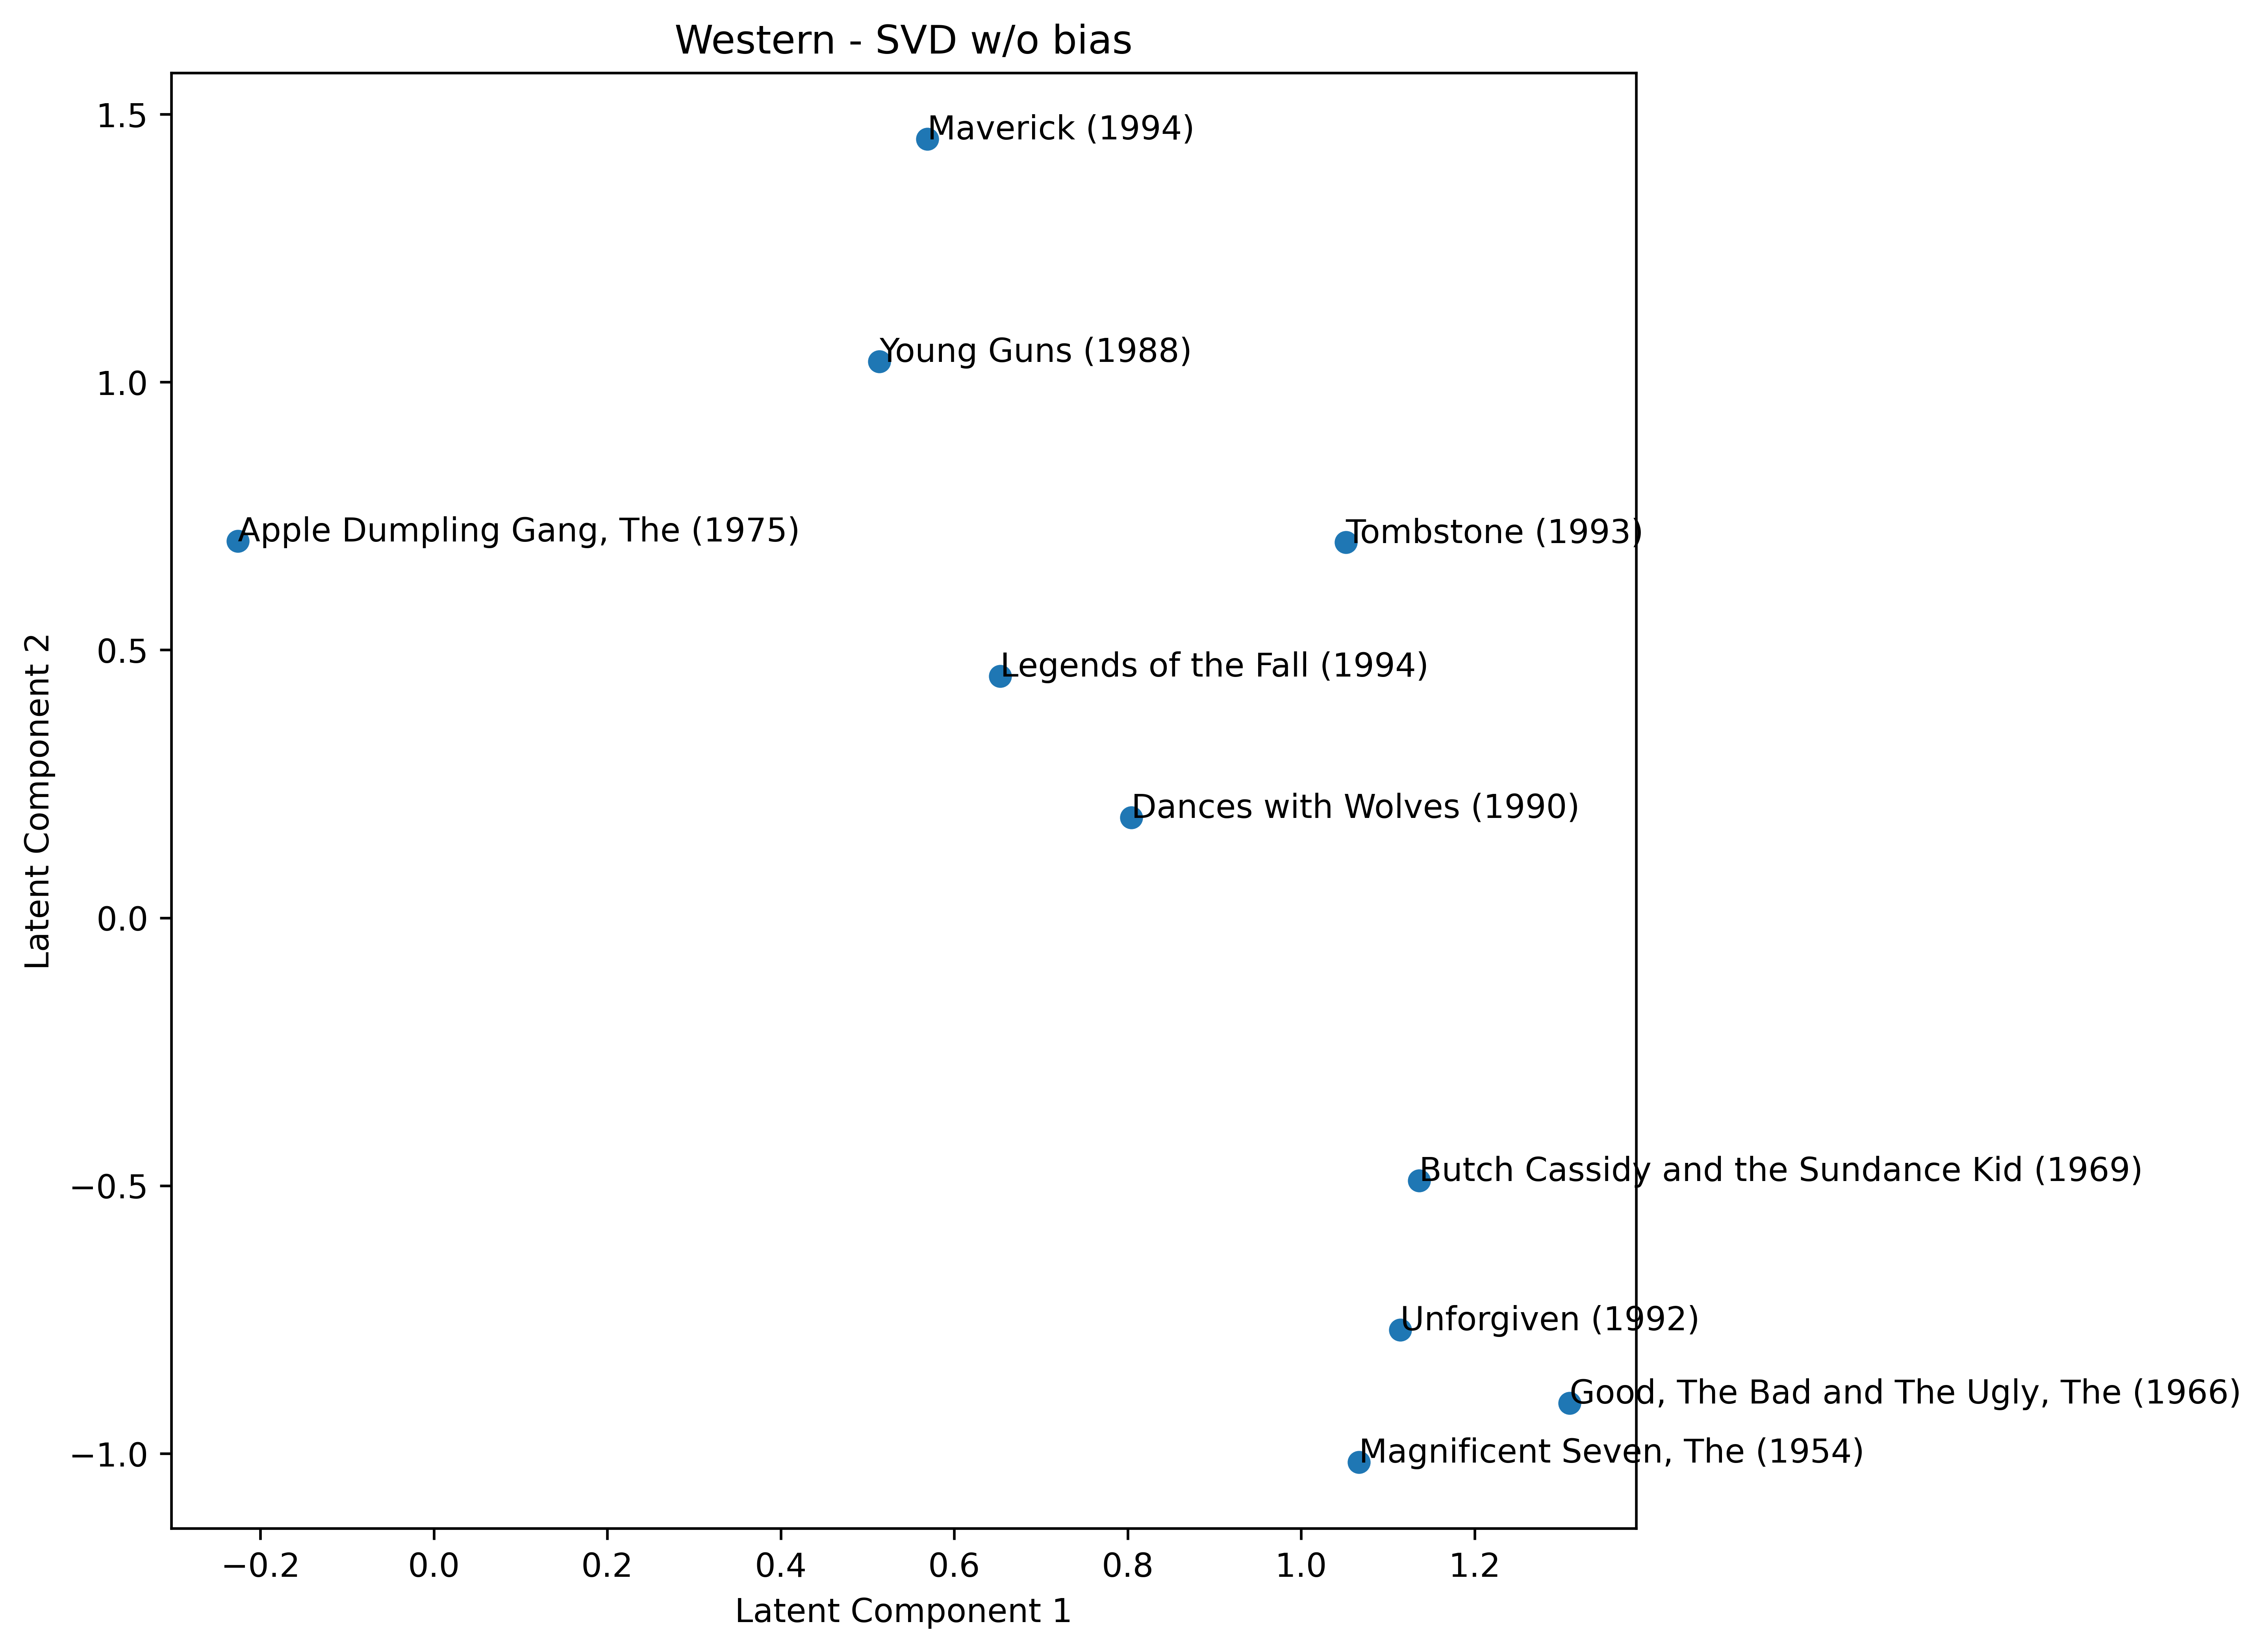
\includegraphics[width = 0.45\textwidth]{western_SVD.png}}
    \subfloat{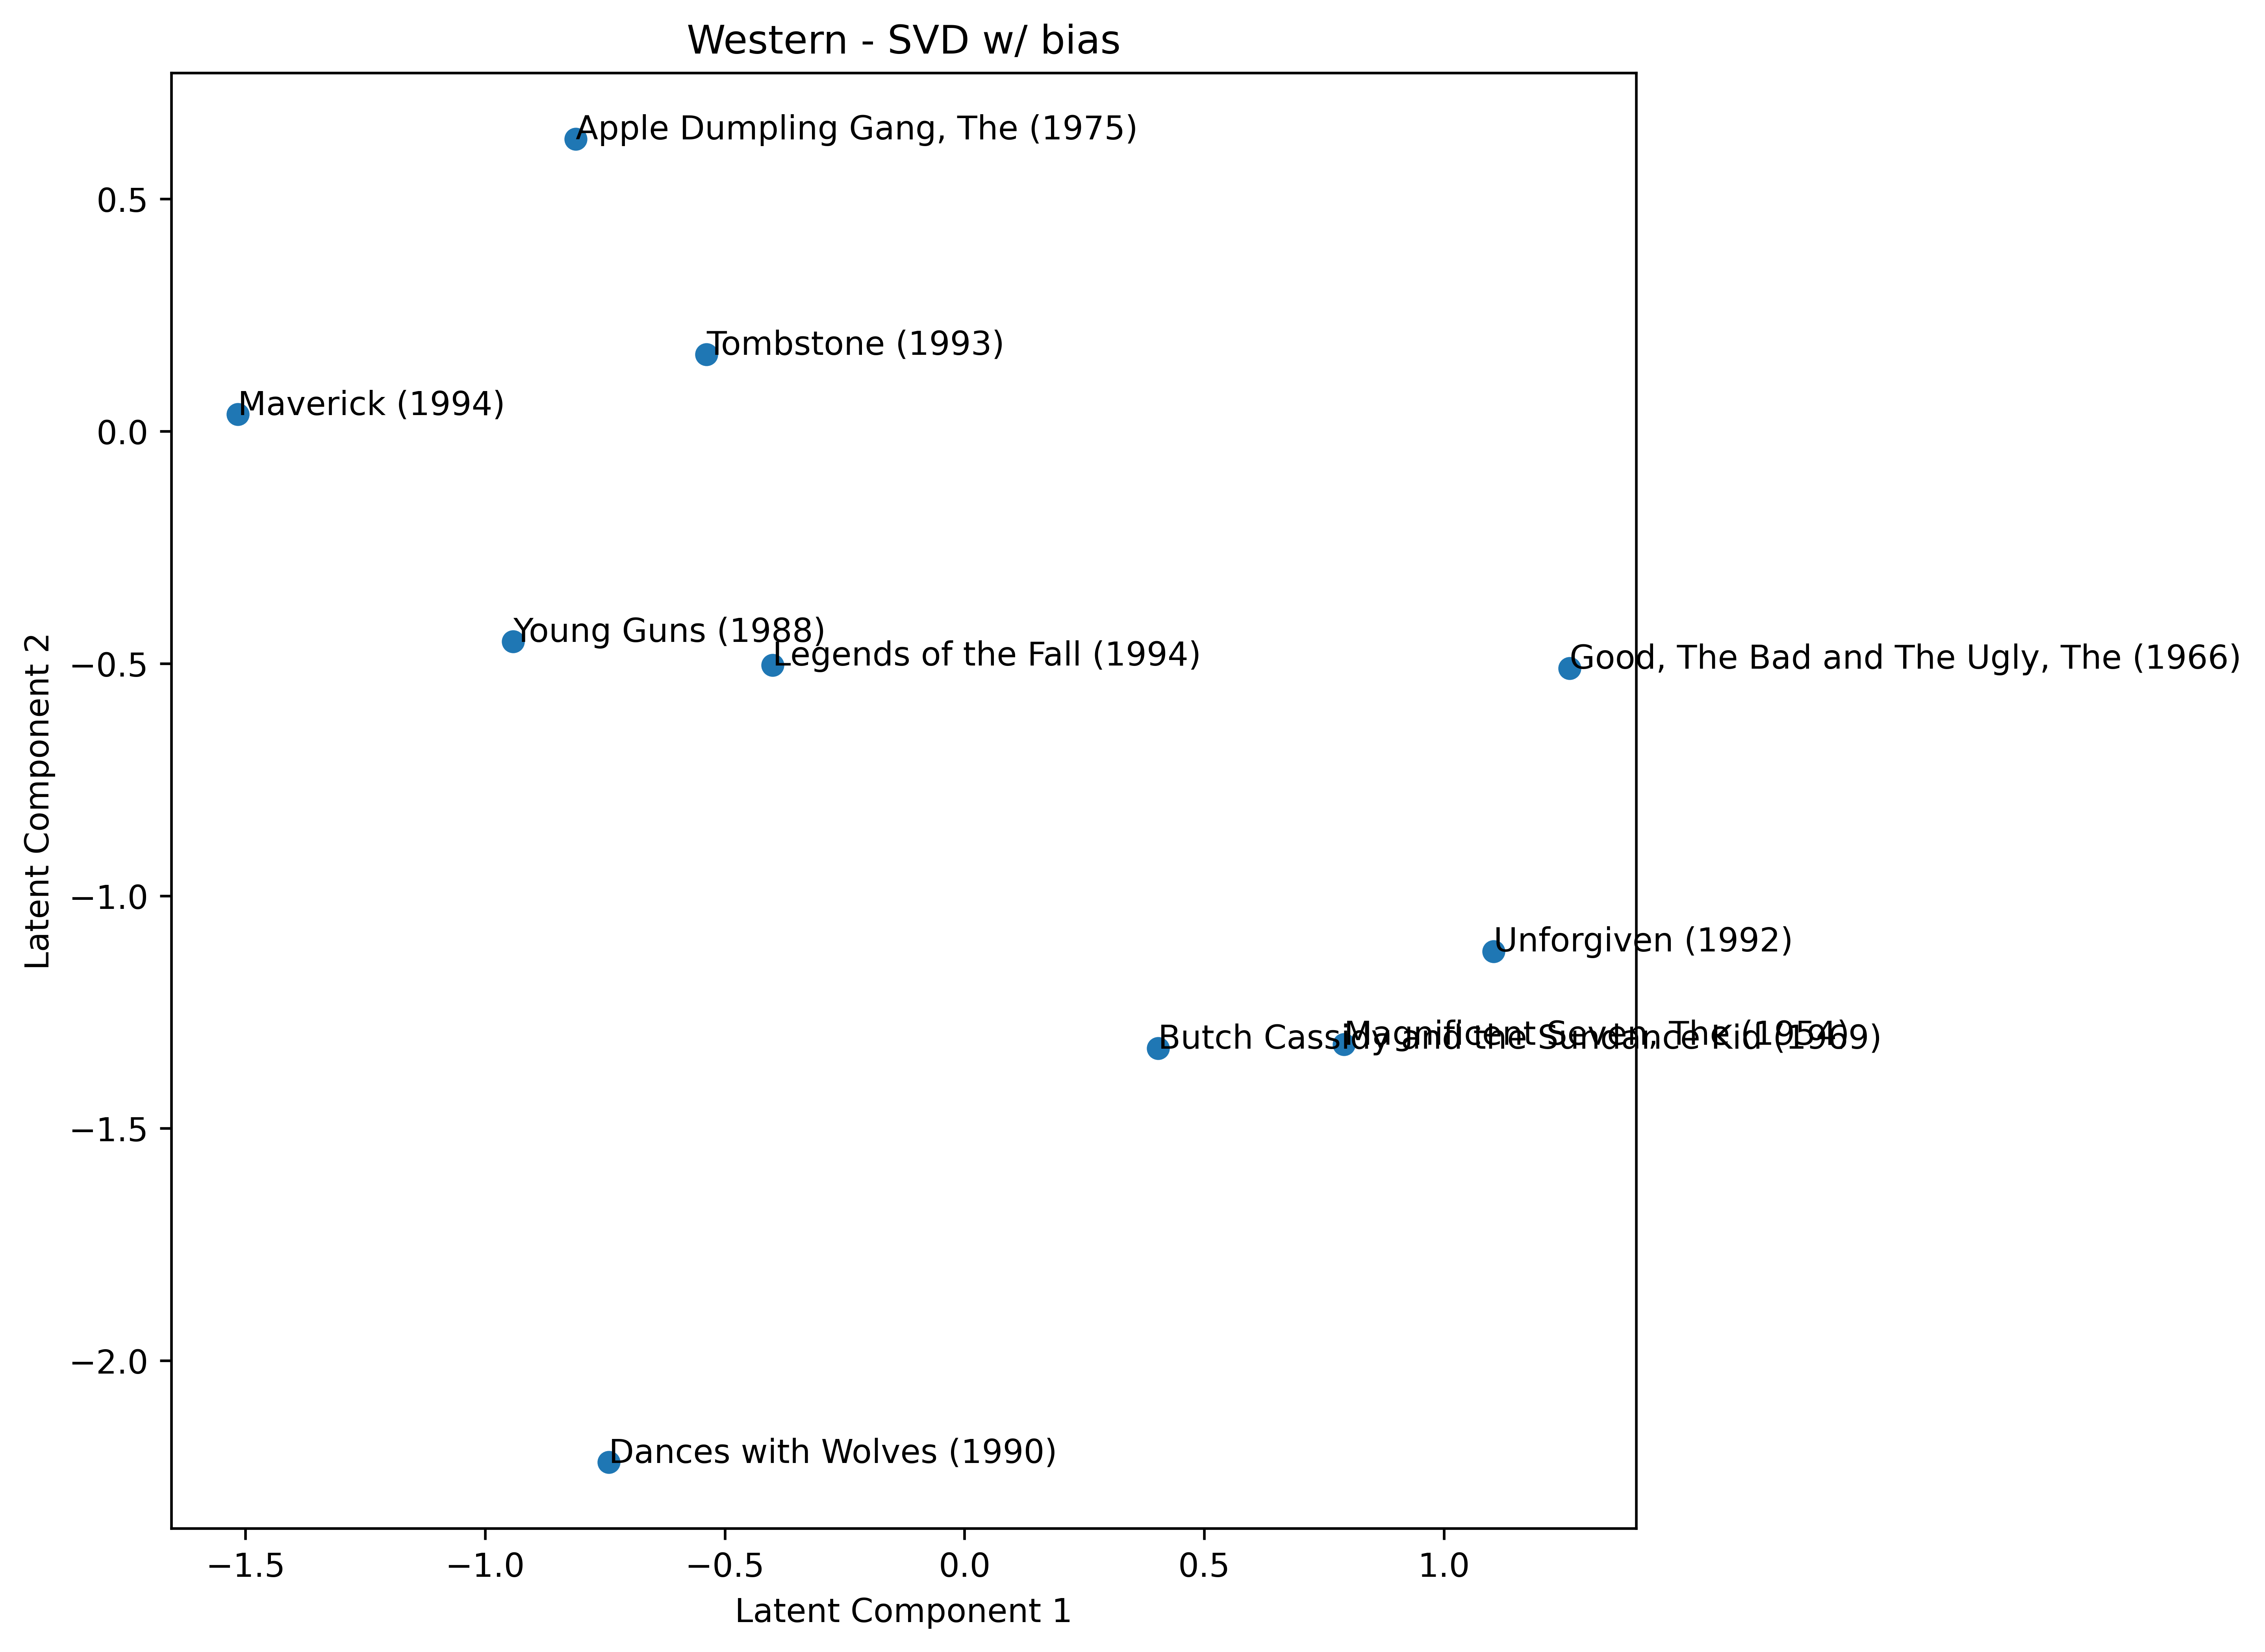
\includegraphics[width = 0.45\textwidth]{western_SVD_biased.png}}
\end{figure}
\begin{figure}[H]
    \centering 
    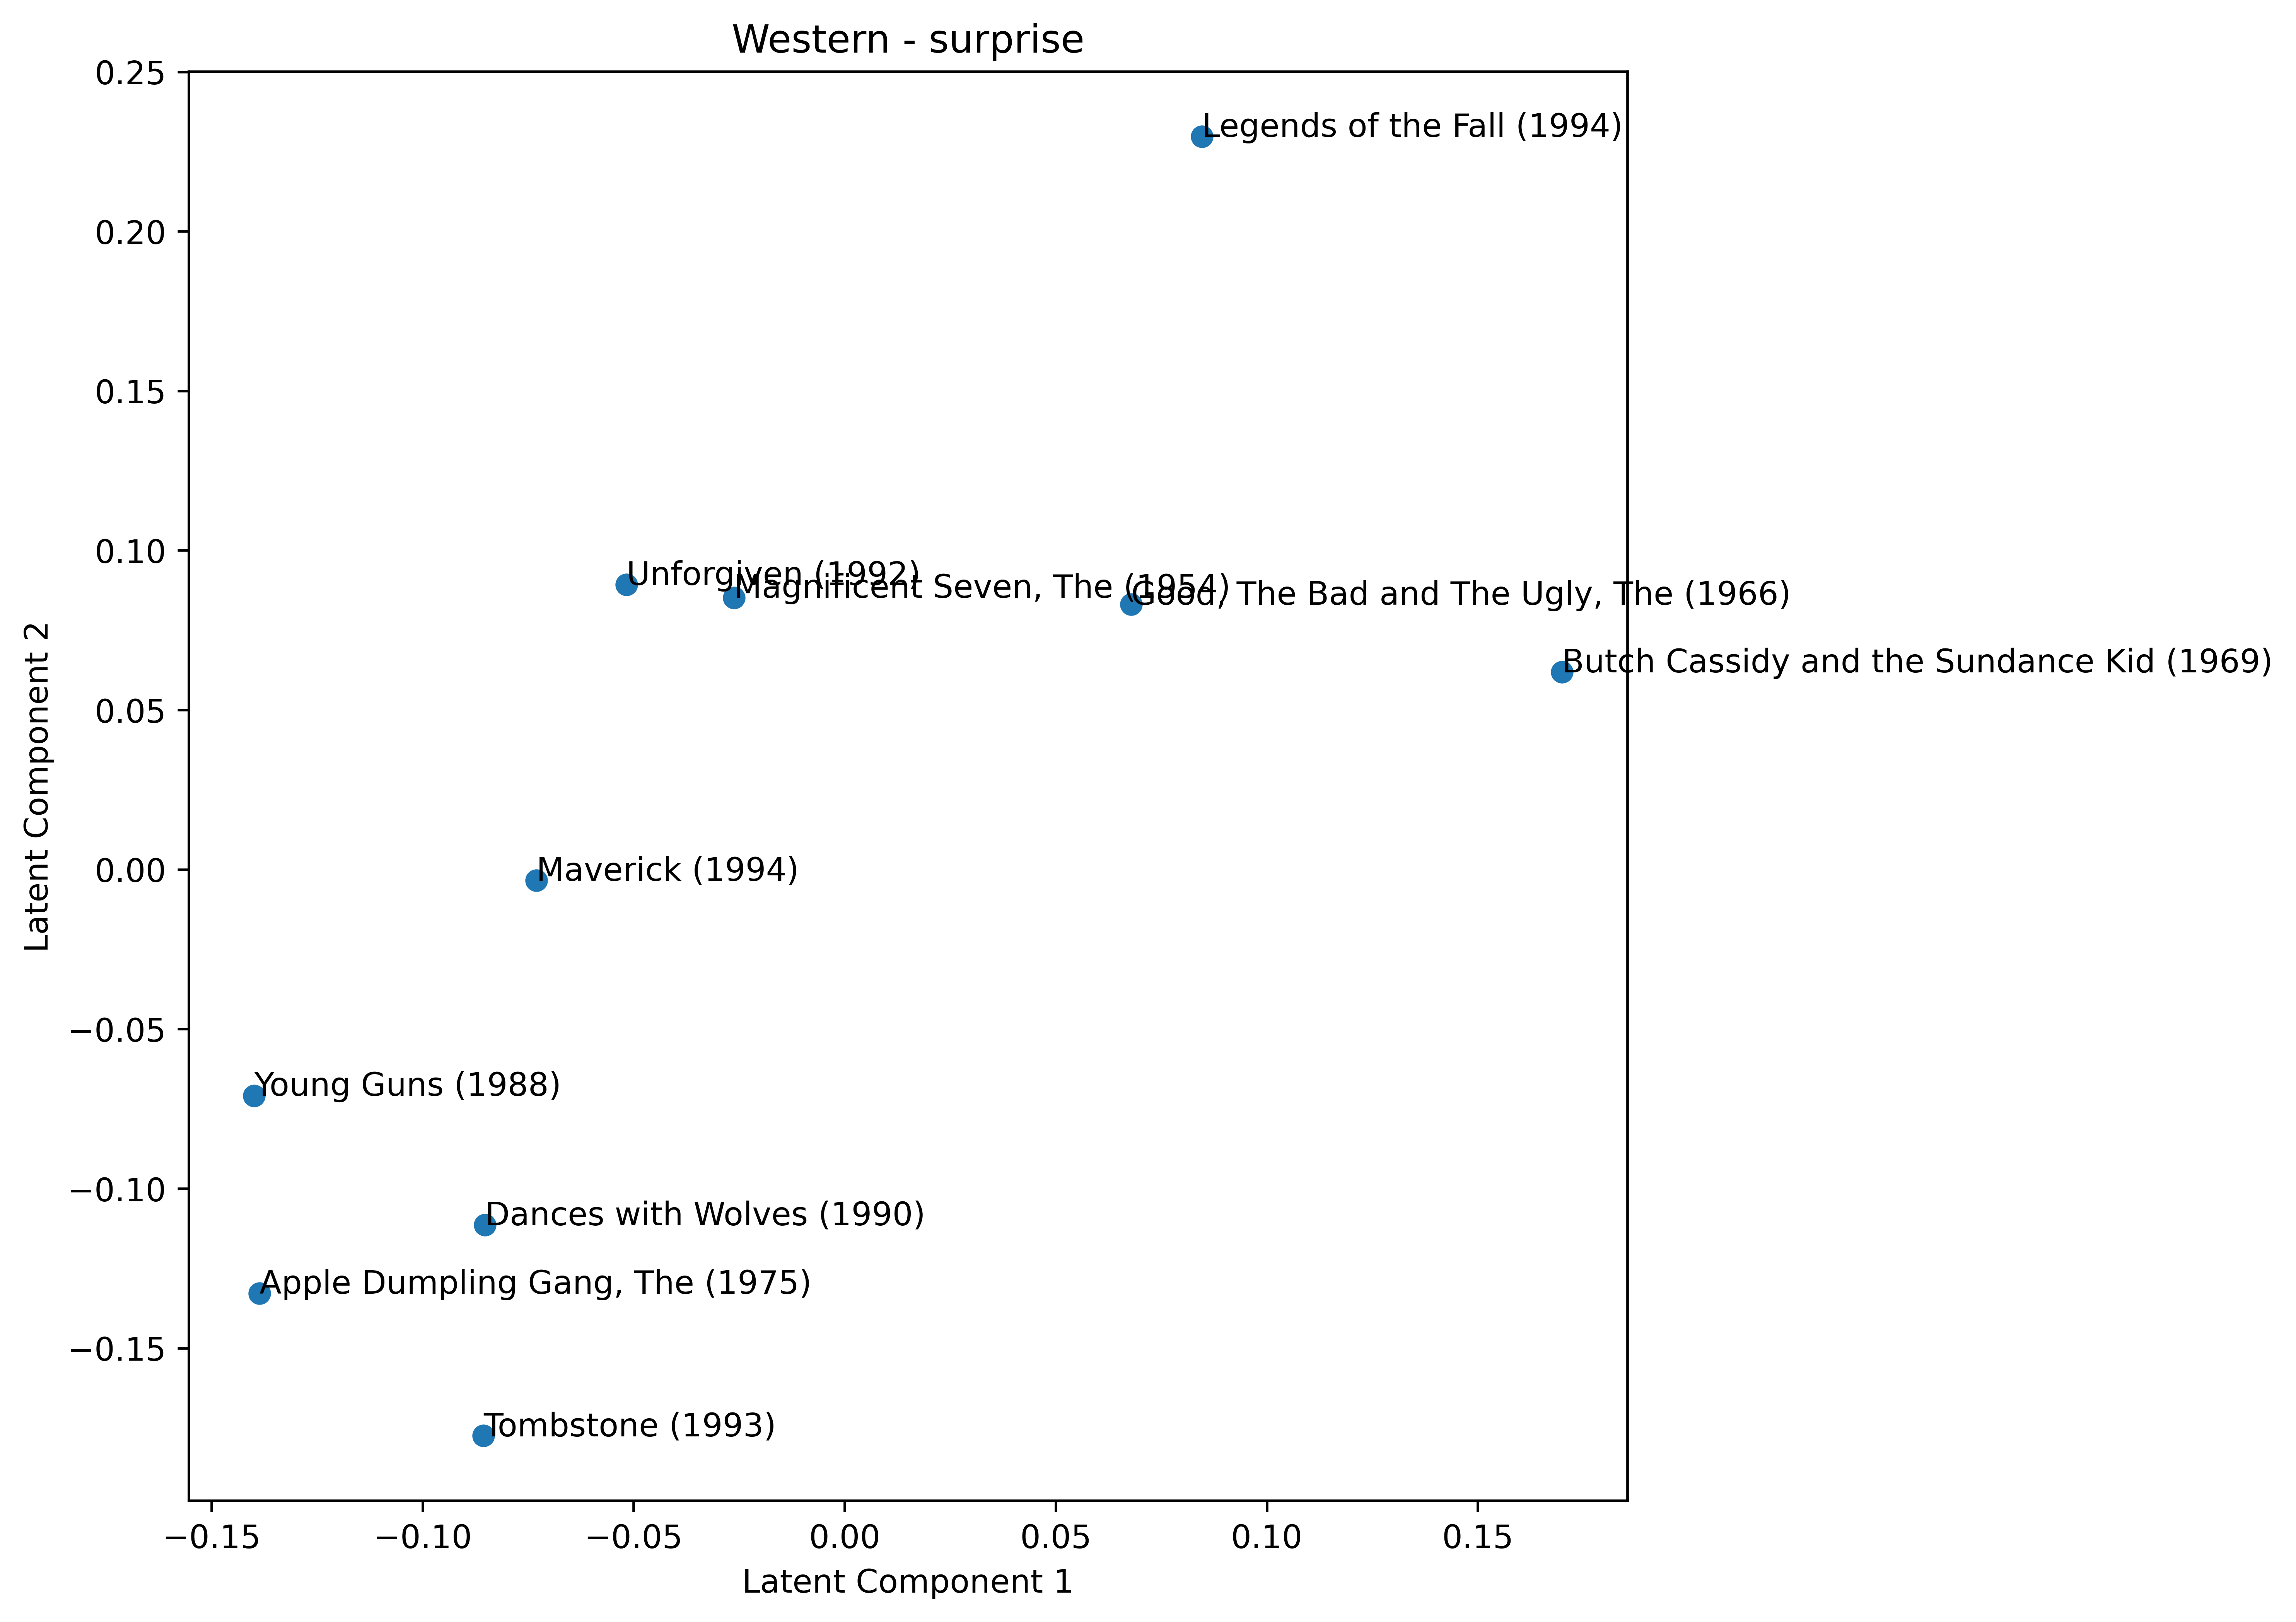
\includegraphics[width=10cm]{western_SVD_sp.png}
\end{figure}

Many Western films are also crime-fiction films which could be why films such as \textit{Unforgiven}, \textit{Butch Cassidy and the Sundance 
Kid}, \textit{The Good, the Bad, and the Ugly}, and \textit{The Magnificent Seven}, are all close to each other in the two SVD plots corresponding 
to our implementation. \textit{The Apple Dumpling Gang} and \textit{Maverick} are also near each other in both of these plots which is also 
reasonable considering that both films have comedy elements.
\par 
The \textit{surprise} implementation makes it's more convincing predictions in this set of films. The films that are clustered together 
in our implementation are also captured by \textit{surprise}.

\newpage

\section{Piazza post}

\url{https://piazza.com/class/m4xf8vvl4206zc/post/220}

\section{LLM Usage}


\end{document}
